% ************************** Thesis Chapter3 **********************************
\chapter{การดำเนินงานวิจัย}
\section{แผนการดำเนินงาน}
การออกแบบหุ่นยนต์ฮิวมานอยด์นั้น ผู้วิจัยได้มีการตั้งชื่อให้หุ่นยนต์ โดยใช้ชื่อว่า อุทัย (UTHAI)
มาจากภาษาอังกฤษคำว่า Universal Template for Humanoid Algorithm Interface
เพื่อให้สมกับเป็นหุ่นยนต์ฮิวมานอยด์ที่ใช้สำหรับงานวิจัยและพัฒนาต่อยอด
การดำเนินงานและการออกแบบการสร้างหุ่นยนต์ฮิวมานอยด์อุทัย มีแผนการทำงานซึ่งแบ่งออกเป็นสามส่วนดังนี้
ส่วนแรกคือ ส่วนของฮาร์ดแวร์ที่เกี่ยวกับโครงสร้างทางกลของหุ่นยนต์ฮิวมานอยด์ เช่น ข้อต่อ ก้านต่อ ฝ่าเท้า
รวมไปถึงระบบอิเล็กทรอนิกส์ ตัวประมวลผลการควบคุม เซนเซอร์ ตัวขับเคลื่อนต่าง ๆ และส่วนที่สองคือ
ส่วนของซอฟท์แวร์ที่เกี่ยวข้องกับการติดต่อสื่อสารกันเบื้องต้น การควบคุมตัวขับเคลื่อนที่ข้อต่อ การอ่านค่าเซนเซอร์
และส่วนที่สาม คือระบบพื้นฐานสำหรับการนำไปศึกษาและพัฒนาต่อยอด

ในการเริ่มต้นทำงานวิจัยเกี่ยวกับฮิวแมนนอยด์นั้นสิ่งจำเป็นที่ต้องทำในอันดับแรกเลยคือการศึกษาสิ่งที่เคยมีอยู่ หรืองานวิจัยได้ทำเอาไว้แล้ว
ศึกษาทำความเข้าใจใน ข้อดี-ข้อเสีย ของวิธีหรือกระบวนการต่างๆ เพื่อนำมาประยุกต์ใช้กับหุ่นยนต์ฮิวมานอยด์ UTHAI เพื่อให้ได้สิ่งที่ดีที่สุด
โดยการศึกษานั้นจะเริ่มต้นจากการศึกษาโครงสร้างทางกลของหุ่นยนต์ฮิวมานอยด์ที่มีอยู่แล้วและมีสิ่งที่ต้องดูเป็นพิเศษคือ
วิธีการเชื่อมต่อกันระหว่างก้านต่อและข้อต่อ, จุดที่ใช้ติดตั้ง IMU และการเลือกใช้วัสดุให้เหมาะสม
รวมถึงการทำงานของเซ็นเซอร์ที่จำเป็นต้องใช้ในการควบคุมการทำงานของหุ่นยนต์ และการทำงานของอุปกรณ์ขับเคลื่อนต่างๆ
เช่น การสั่งงานมอเตอร์ Digital servo ผ่าน Protocol ของ Dynamixel

\clearpage
\section{การออกแบบโครงสร้างของหุ่นยนต์}
การออกแบบทางโครงสร้างทางกลของหุ่นยนต์ฮิวมานอยด์ UTHAIนั้น ผู้วิจัยได้เลือกใช้โปรแกรมออกแบบโครงสร้างเป็นโปรแกรม Solidworks
ที่ช่วยในการพัฒนาแบบจำลองของหุ่นยนต์ฮิวมานอยด์ UTHAI
เนื่องจากโปรแกรม Solidworks เป็นโปรแกรมที่ใช้ในการออกแบบ วาดแบบทางวิศวกรรม
สามารถวิเคราะห์โครงสร้างการรับแรงของแบบจำลองได้ อีกทั้งยังเป็นเครื่องมือที่มีการใช้งานอย่างแพร่หลาย
ทำให้สามารถดาวน์โหลดแบบจำลองต่างๆที่มีคนพัฒนาเข้าเข้ามาใช้ร่วมกับการออกแบบได้ 
และด้วยทางผู้วิจัยมีความคำนึงถึงการพัฒนาต่อยอดเป็นหลัก ดังนั้นการออกโครงสร้างทางกลของหุ่นยนต์ฮิวมานอยด์ UTHAI
จึงถูกออกแบบมาเพื่อให้สามารถรองรับการปรับเปลี่ยน เปลี่ยนแปลง แก้ไขชิ้นส่วนต่างๆของตัวหุ่นยนต์ฮิวมานอยด์ UTHAIได้

\subsection{โครงสร้างหุ่นยนต์}
หุ่นยนต์ที่สร้างขึ้นประกอบด้วยส่วนของลำตัวและส่วนขา ในขาแต่ละข้างออกแบบให้เป็นลักษณะของข้อต่อหมุน (Revolute joint)
เลียนแบบโครงสร้างของมนุษย์ซึ่งประกอบด้วย ส่วนของสะโพกที่มีองศาอิสระจำนวน 3 องศาอิสระ ส่วนของหัวเข่า 1
องศาอิสระและส่วนของข้อเท้า 2 องศาอิสระ รวมขาข้างละ 6 องศาอิสระ ระบบต้นกำลังที่ใช้เป็น Dynamixel servo การออกแบบหุ่นยนต์นั้น
สิ่งแรกที่ต้องทำ คือ การกำหนดโครงสร้างของข้อต่อและก้านต่อขึ้นมาก่อน โดยวาดขึ้นมาเป็นเหมือนโครงกระดูก
ซึ่งโครงสร้างนั้นทางผู้วิจัยได้อ้างอิงมาจากสัดส่วนของมนุษย์จริง ที่ประกอบด้วยส่วนของขาข้างละ 6 องศาอิสระ และมีจุดศูนย์กลาง
อยู่บริเวณกระดูกเชิงกรานของตัวหุ่นยนต์เอง
\begin{figure}[!ht]
    \centering
    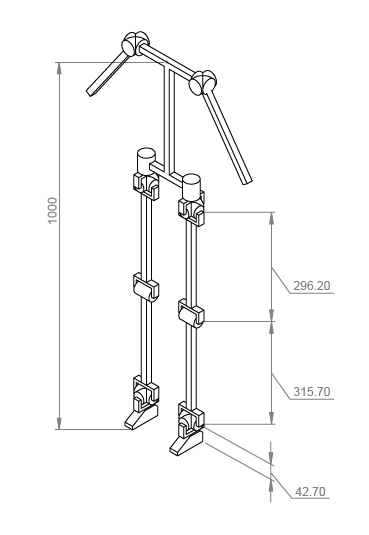
\includegraphics[width=0.35\textwidth]{chapter3/images/uthai_structure1.png}
    \caption{ภาพแสดงแสดงโครงสร้างของหุ่นยนต์ UTHAI}
    \label{fig:uthai_structure1}
\end{figure}

เมื่อเราได้แบบจำลองของหุ่นยนต์ฮิวมานอยด์ออกมาแล้ว ลำดับต่อไปคือการกำหนดตำแหน่งการติดตั้งเซนเซอร์และตัวขับเคลื่อนต่างๆเข้าไป
โดยมี Ground contact sensor ติดตั้งที่ใต้ฝ่าเท้าของหุ่นยนต์, IMU sensor ติดตั้งไว้ให้ใกล้กับจุด COM ของหุ่นยนต์ และ Dynamixel servo
ติดตั้งไว้ที่ข้อต่อในแต่ละข้อต่อ

\begin{figure}[!ht]
    \centering
    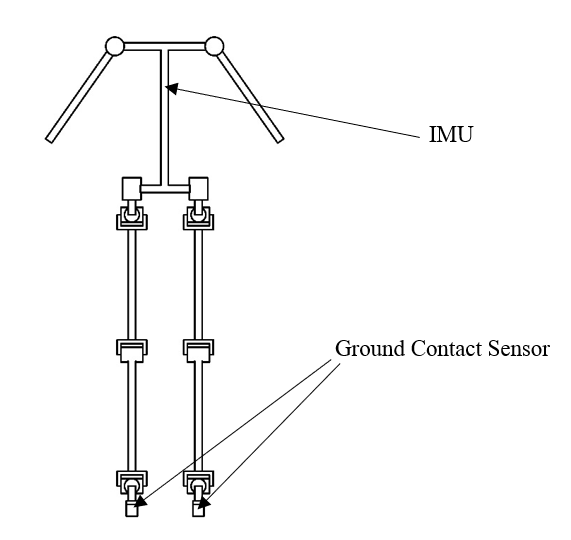
\includegraphics[width=0.5\textwidth]{chapter3/images/uthai_sensor.PNG}
    \caption{ภาพแสดงการติดตั้งเซนเซอร์ในจุดต่างๆ}
    \label{fig:uthai_structure2}
\end{figure}

ส่วนโครงสร้างหุ่นยนต์ฮิวมานอยด์ UTHAI ทางผู้วิจัยเลือกใช้วัสดุหลักเป็น PLA ที่ขึ้นรูปด้วยวิธีการขึ้นรูปสามมิติ
และมีวัสดุเสริมบางชิ้นส่วนจากอลูมิเนียม เนื่องจากจะทำให้โครงสร้างมีน้ำหนักเบา สามารถปรับปรุงแก้ไขง่าย และมีราคาที่สมเหตุสมผล
\begin{table}[ht]
	\centering
	\begin{tabular}{| l | l | l |}
		\hline
		Material & Longitudinal Tensile Strength ($ksi$) & Density ($g/cm^3$) \\
        \hline
        Carbon Fiber & 300 & 1.55 \\
        Steel & 100	& 7.7 \\
        Titanium & 120 & 4.34 \\
        Aluminum & 35 & 2.7 \\
        PLA 3D printing (50 \% infill) & 3.5 & 1.26 \\
        PLA 3D printing (100 \% infill) & 5.5 & 1.26 \\
	    \hline
	\end{tabular}
	\caption{ตารางแสดงสมบัติทางกลของวัสดุต่าง ๆ}
	\label{tab:material_properties}
\end{table}

\clearpage
\subsection{จัดทำชิ้นส่วนโครงสร้างและประกอบ}
ในกาารจัดทำชิ้นส่วนโครงสร้างนั้นทางผู้จัดทำได้คำนึงถึงความแข็งแรงเป็นหลักซึ่งมีความสำคัญมาก
ในการเคลื่อนที่ของหุ่นยนต์ และยังคงต้องมีน้ำหนักที่เบาอีกด้วย\footnote{ Printing Guide [https://filaments.ca/pages/temperature-guide]}
ดังนั้นจึงได้ใช้การขึ้นรูปชิ้นงานด้วยเทคนิค
การพิมพ์ 3 มิติ โดยจะใช้วัสดุหลักเป็นพลาสติก PLA ซึ่งมีความแข็งมากกว่าและขึ้นรูปง่ายกว่าพลาสติกชนิด ABS
เพื่อให้ตอบโจทย์กับหุ่นยนต์แพลตฟอร์มเพื่อพัฒนาต่อยอดในอนาคต ซึ่งผู้ใช้ทุกคนสามารถพิมพ์ขึ้นมาได้ด้วยตนเอง\footnote{ PLA vs ABS [https://www.3dhubs.com/knowledge-base/pla-vs-abs-whats-difference]}

\begin{table}[ht]
	\centering
	\begin{tabular}{| l | l | l |}
		\hline
		Properties & ABS & PLA \\
        \hline
        Tensile Strength & 27 $MPa$ & 37 $MPa$ \\
        Elongation & 3.5 \- 50\% & 6\% \\
        Flexural Modulus & 2.1 \- 7.6 $GPa$ & 4 $GPa$ \\
        Density & 1.0 - 1.4 $g/cm^3$ & 1.3 $g/cm^3$ \\
        Melting Point & 230$°C$ - 240$°C$ & 215$°C$ - 235$°C$ \\ 
        การย่อยสลายทางธรรมชาติ & ไม่ได้ & ได้ (ภายใต้เงื่อนไขที่ถูกต้อง) \\
	    \hline
	\end{tabular}
	\caption{ตารางแสดงสมบัติทางกลของวัสดุพลาสติก}
	\label{tab:plastic_material_properties}
\end{table}
แต่เนื่องจากว่าในปัจจุบันนี้เครื่องพิมพ์ส่วนมากจะไม่รองรับการพิมพ์ชิ้นงานที่มีขนาดใหญ่ ซึ่งมีขนากมากกว่า
30x30x30 ซม. (กว้างxยาวxสูง) ดังนั้นชิ้นงานที่ขึ้นรูปที่มีขนาดใหญ่เกินกว่านี้อาจจะต้องทำการตัดชิ้นงานออกก่อน
แล้วจึงค่อยนำมาประกอบรวมกันทีหลังอีกครั้งหนึ่ง โดยพื้นที่ทำการพิมพ์ของเครื่องพิมพ์ 3 มิติที่มีวางจำหน่าย
และใช้งานแพร่หลายในท้องตลาดแสดงดังตาราง\ref{tab:3dprint_space} \footnote{The truth about 3D printer maximum print areas [https://www.zdnet.com/article/what-manufacturers-dont-want-you-to-know-the-truth-about-3d-printer-maximum-print-areas/]}

\begin{table}[ht]
	\centering
	\begin{tabular}{| l | l | l | l |}
		\hline
		Printer & Actual Width & Actual Depth & Actual Height \\
        \hline
        MakerBot Replicator+ & 292 & 192 & 165 \\
        Ultimaker 3 & 188 & 185 & 200 \\
        LulzBot Mini & 152 & 152 & 158 \\
        Dreammaker Overlord Pro Plus & 79 & 79 & 255 \\
        New Matter MOD-t & 145 & 95 & 125 \\
	    \hline
	\end{tabular}
	\caption{ตารางแสดงขนาดของชิ้นงานที่สามารถพิมพ์ได้ในเครื่องพิมพ์ชนิดต่างๆ}
	\label{tab:3dprint_space}
\end{table}





%%%%%%%%%%%%%%%%%%%%%%%%%%%%%%%%%%%%%%%%%%%%%%%%%%%%%%%%%%%%%%%%%%%%%%%%%%%%%%%
%%%%%%%%%%%%%%%%%%%%%%%%%%%%%%%%%%%%%%%%%%%%%%%%%%%%%%%%%%%%%%%%%%%%%%%%%%%%%%%
%%%%%%%%%%%%%%%%%%%%%%%%%%%%%%%%%%%%%%%%%%%%%%%%%%%%%%%%%%%%%%%%%%%%%%%%%%%%%%%
\clearpage
\subsection{อุปกรณ์ที่ใช้ในหุ่นยนต์ฮิวมานอยด์ UTHAI}

\subsubsection*{Dynamixel servo EX-106+}
Dynamixel EX-106+ เป็นตัวขับเคลื่อนที่นิยมใช้ในปัจจุบัน ซึ่งเป็นเซอร์โวมอเตอร์ที่เหมาะสำหรับทำหุ่นยนต์โดยเฉพาะ
ภายในประกอบไปด้วย มอเตอร์กระแสตรง ชุดเฟืองมอเตอร์ ไดรเวอร์คอนโทรเลอร์ สามารถเชื่อมต่อกันผ่าน BUS RS-485
\footnote{ Robot Actuator [http://support.robotis.com/en/product/actuator/dynamixel/ex\_series/ex-106.htm] }
มีการควบคุมแบบ PID สามารถที่จะอ่านค่าความเร็ว
แรงดันไฟฟ้า กระแสไฟฟ้า อุณหภูมิ ตำแหน่ง และแรงบิดจากมอเตอร์ทุกตัวได้ แต่ละมอเตอร์แต่ละตัวจะมีบอร์ดควบคุมของตัวเอง
เราสามารถที่จะจ่ายไฟให้มอเตอร์และควบคุมผ่าน Serial ได้เลย

การทำงานของตัวขับเคลื่อนนี้สามารถทำได้ 2 รูปแบบคือ\footnote{ EX-106+ Mode [http://www.trossenrobotics.com/dynamixel-ex-106-robot-actuator.aspx] }

\paragraph*{Joint Mode}
สามารถที่จะควบคุม Torque Speed และ position ได้ความละเอียดในการควบคุม 10-bit (0-1023) หมุนได้อยู่ในช่วง 0-250 องศา

\paragraph*{Wheel Mode}
สามารถที่จะควบคุม Torque Speed และ direction ได้ ความละเอียดของความเร็วมอเตอร์เท่ากับ 10bit (0-1023) สามารถหมุนได้ครบ 360 องศาได้

\begin{figure}[!ht]
    \centering
    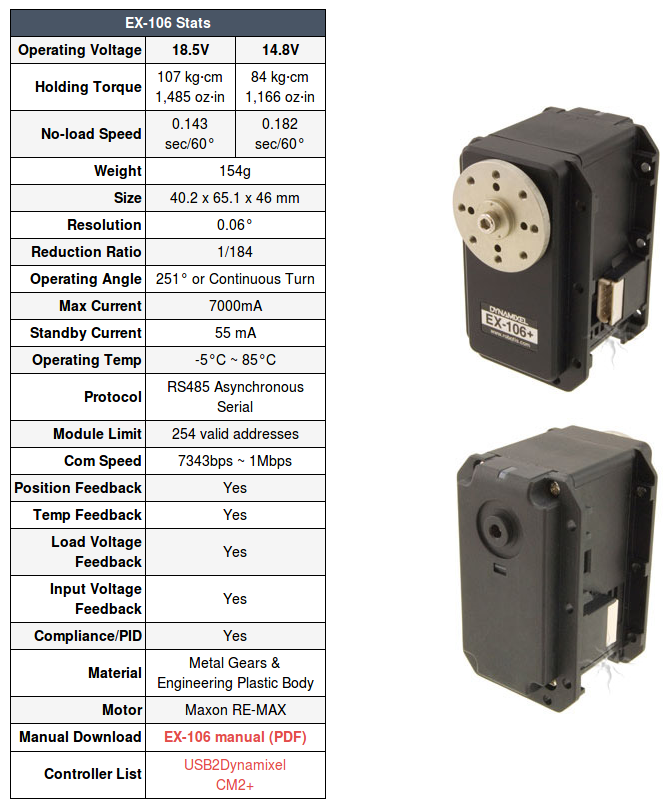
\includegraphics[width=0.75\textwidth]{chapter3/images/dxl_ex106.png}
    \caption{แสดงประสิทธิภาพของมอเตอร์ EX-106+}
    \label{fig:dxl_ex106}
\end{figure}


\clearpage
\subsubsection*{USB2Dynamixel connector}
USB2Dynamixel เป็นอุปกรณ์สำหรับเชื่อมต่อหน่วยประมวลผลระดับสูง (Odroid) กับดิจิตอลเซอร์โวโดยจะเชื่อมต่อ ผ่านพอร์ท USB ของ Odroid ไปยังดิจิตอลเซอร์โว
ผ่านสาย 2 เส้น คือ D+ และ D-
เป็นการเชื่อมต่อแบบ RS-485\footnote{USB2Dynamixel [http://support.robotis.com/en/product/auxdevice/interface/usb2dxl\_manual.html]}
ืทำให้สามารถส่งข้อมูลระยะทางไกลได้ และสามารถที่จะมีหลายอุปกรณ์บนสายเส้นเดียวกันได้

\begin{figure}[!ht]
    \centering
    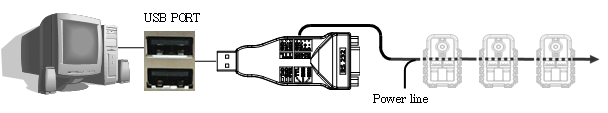
\includegraphics[width=0.75\textwidth]{chapter3/images/dynamixel2pc.png}
    \caption{ภาพแสดงการติดต่อสื่อสารระหว่างคอมพิวเตอร์กับมอเตอร์ Dynamixel}
    \label{fig:dynamixel2pc}
\end{figure}

ในการต่อใช้งานนั้นผู้ใช้งานจำเป็นต้องเลือกการติดต่อสื่อสารระหว่าง คอมพิวเตอร์กับมอเตอร์
ซึ่งการติดต่อสื่อสารนั้นหากใช้ USB2Dynamixel ตัวอุปกรณ์ชิ้นนี้ได้แบ่งการติดต่อสื่อสารออกเป็น 3 รูปแบบคือ
\vspace{-10pt}
\begin{enumerate}[label=\arabic*, leftmargin=1.5cm]
    \setlength\itemsep{-0.25em}
    \item TTL Communication : สำหรับดิจิตอลเซอร์โวที่ใช้พอร์ทชนิด 3-pin เช่นในตระกูล AX Series เช่น AX-S1 AX-12+ ฯลฯ
    \item RS485 Communication : สำหรับดิจิตอลเซอร์โวที่ใช้พอร์ทชนิด 4-pin เช่นในตระกูล DX Series เช่น RX Series, EX Series ฯลฯ
    \item RS232 Communication : ใช้สำหรับติดต่อสื่อสารกับคอนโทรลเลอร์ผ่านสายเคเบิล
\end{enumerate}
\vspace{-15pt}
\begin{figure}[!ht]
    \centering
    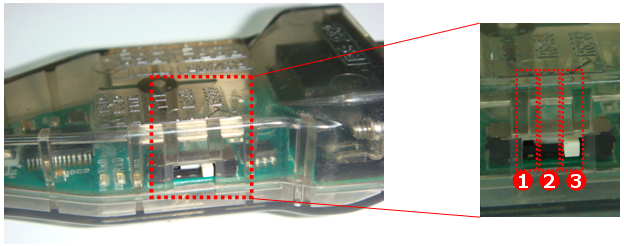
\includegraphics[width=0.5\textwidth]{chapter3/images/useusb2dynamixel.png}
    \caption{ภาพแสดงการเลือกโหมดใช้งานของ USB2Dynamixel}
    \label{fig:useusb2dynamixel}
\end{figure}

แต่จากการทดลองนำมาใช้ผู้วิจัยพบว่า Dynamixels ที่ใช้ในการทำงานวิจัยครั้งนี้เป็นชนิด 4 pin ซึ่งใช้ RS485 ในการติดต่อสื่อสาร
และด้วยขนาดของตัว USB2Dynamixel มีขนาดที่ใหญ่ทำให้การทำงานมีความลำบากในการติดตั้งลงบนตัวของหุ่นยนต์
จึงได้ทำการเปลี่ยนเป็น USB to RS485 แทน
\begin{figure}[!ht]
    \centering
    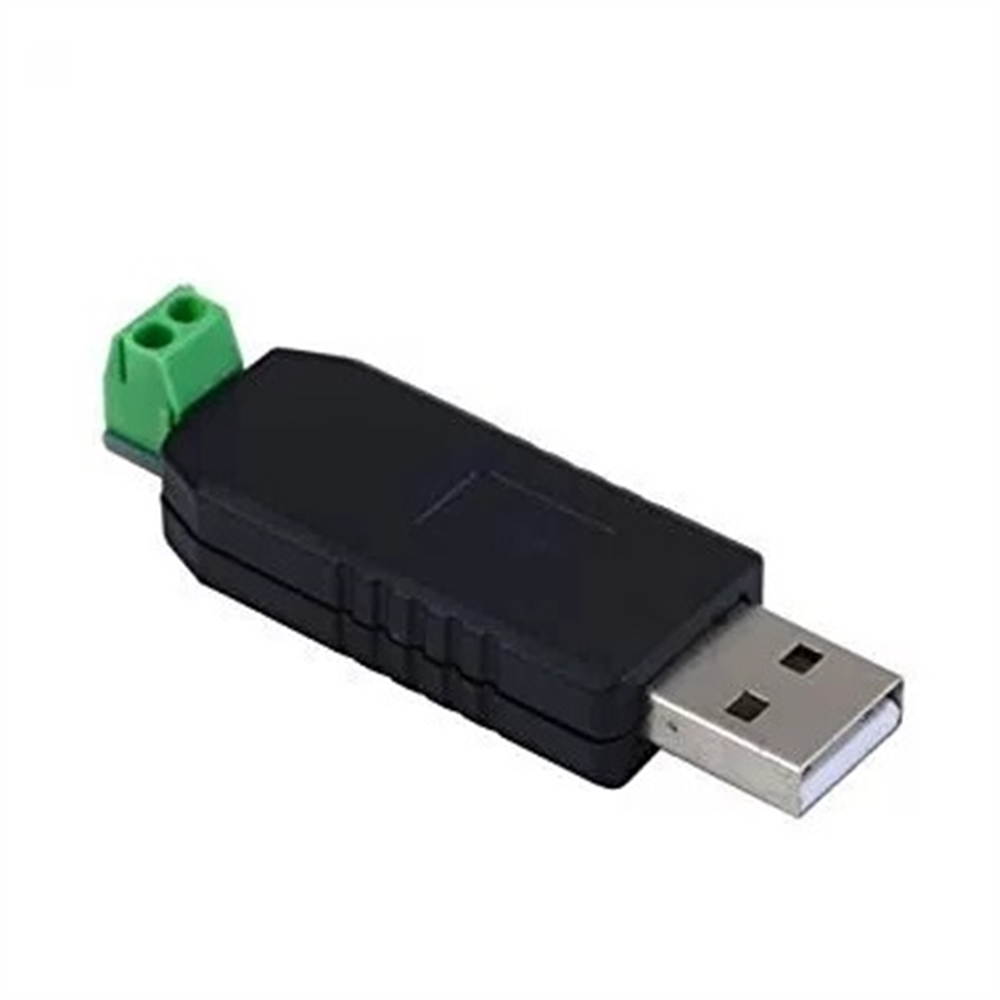
\includegraphics[width=0.3\textwidth]{chapter3/images/usb2rs485.jpg}
    \caption{USB2RS485 Module}
    \label{fig:usb2rs485}
\end{figure}

\clearpage
\subsubsection*{Inertial Measurement Unit (IMU)}
ในการทำวิจัยครั้งนี้ผู้จัดทำได้เลือกนำเซนเซอร์ MPU-9250 มาใช้ในการอ่านค่ามุมเอียงของหุ่นยนต์เพื่อใช้ในการคุมเสถียรภาพของหุ่นยนต์
โดยเซนเซอร์ตัวนี้สามารถวัดค่าได้ 9 แกนคือ วัดค่าความเร็วเชิงมุม (gyroscope) 3 แกน วัดค่าความเร่งเชิงเส้น(accelerometer) 3 แกน
และวัดค่าสนามแม่เหล็กโลก (magnetometer) 3 แกน ซึ่งเซนเซอร์ตัวนี้จะติดตั้งบริเวณส่วนของลำตัวหุ่นยนต์
เนื่องจากว่าจะเป็นจุดที่สามารถบ่งบอกได้ถึงการเคลื่อนที่และมุมเอียงของหุ่นยนต์ในขณะนั้นได้ดีที่สุด\footnote{ MPU-9250 [http://www.arduiner.com/en/gy-series-axis-accellerometers/6924-gy9255-mpu9255-sensor-module-alternative-mpu9150-mpu9250-3809200640200.html] }
\begin{figure}[!ht]
    \centering
    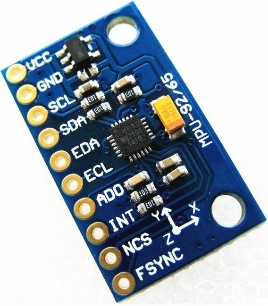
\includegraphics[width=0.2\textwidth]{chapter3/images/mpu9250.jpeg}
    \caption{แสดงเซนเซอร์ IMU MPU9250}
    \label{fig:mpu9250}
\end{figure}

\subsubsection*{Wi-Fi Adapter}
ตัวรับสัญญาณ wifi ชนิดพกพาเพื่อใช้ในการติดต่อสื่อสารระหว่างคอมพิวเตอร์ที่ติดตั้งอยู่บนตัวของหุ่นยนต์
และคอมพิวเตอร์ที่เป็นตัวสั่งการซึ่งอยู่นอกตัวของหุ่นยนต์ ซึ่งในงานวิจัยนี้
จะใช้ส่งข้อมูลที่ได้หลังจากการประมวลผลบนคอมพิวเตอร์ไปยังตัวหุ่นยนต์ เช่น การวางแผนการเดิน การคำนวนพลศาสตร์ของหุ่นยนต์
และอื่นๆ โดยการส่งข้อมูลไปยังคอมพิวเตอร์ที่อยู่บนตัวหุ่นยนต์นั้นจะมีตัวกลางในการรับส่งสัญญาณ
คือ ตัวกระจายสัญญาณ (wifi router)
\begin{figure}[!ht]
    \centering
    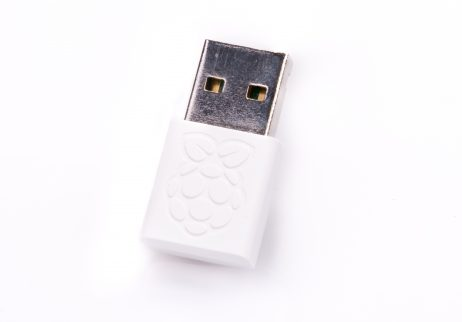
\includegraphics[width=0.3\textwidth]{chapter3/images/rpi_wifi_adaptor.jpg}
    \caption{ตัวรับสัญญาณ wifi ของ RaspberryPi}
    \label{fig:rpi_wifi_adaptor}
\end{figure}
\begin{figure}[!ht]
    \centering
    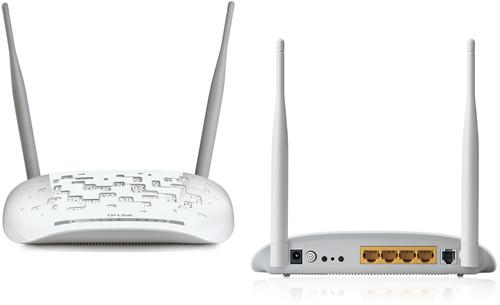
\includegraphics[width=0.3\textwidth]{chapter3/images/wifi_router.jpg}
    \caption{ตัวกระจายและรับส่งสัญญาณ wifi}
    \label{fig:wifi_router}
\end{figure}


\clearpage
\subsubsection*{Ground contact sensor}
เซนเซอร์ตรวจหน้าสัมผัสที่พื้นเป็นเซนเซอร์ที่ถูกติดตั้งบริเวณฝ่าเท้า เพื่อตรวจสอบการเดินของหุ่นยนต์ฮิวมานอยด์ว่าขณะนี้มีการสัมผัสของฝ่าเท้าของหุ่นยนต์กับพื้นหรือไม่ 
ซึ่งในงานวิจัยนี้ได้ใช้หลักการตัวตรวจจับแรงกดแบบค่าความต้านทานหรือ Force Sensing Resistor (FSR) ที่ใช้เทคโนโลยีฟิล์มโพลีเมอร์แบบหนา (Polymer Thick Film) 
โดยแรงดันไฟฟ้าที่ตกคร่อมตัวตรวจจับจะลดลง เมื่อมีแรงกดมากระทำบนแผ่นตรวจจับ มีโครงสร้างของตัวตรวจจับแสดง ดังรูปที่ \ref{fig:FSRarchitec}
\begin{figure}[!ht]
    \centering
    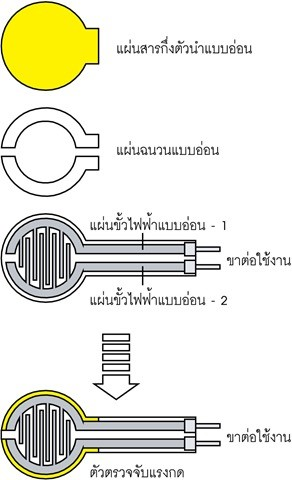
\includegraphics[width=0.35\textwidth]{chapter3/images/FSRarchitec.jpg}
    \caption{ลักษณะโครงสร้างของตัวตรวจจับแรงกด FSR}
    \label{fig:FSRarchitec}
\end{figure}

ประกอบด้วยแผ่นสารกึ่งตัวนำแบบอ่อนที่เป็นตัวกำหนดค่าความต้านทานไฟฟ้าประกบ เข้ากับแผ่นขั้วไฟฟ้าแบบอ่อน โดยมีแผ่นฉนวนแบบอ่อนคั่นกลาง 
ทำให้เกิดค่าความต้านทานไฟฟ้าขึ้นระหว่างขาต่อใช้งาน เมื่อมีการกดลงบนแผ่นขั้วนำไฟฟ้า จะทำให้เกิดการสัมผัสระหว่างสารกึ่งตัวนำกับขั้วไฟฟ้า
ส่งผลให้ค่าความต้านทานไฟฟ้าเกิดการเปลี่ยนแปลง ดังแสดงกระบวนการทำงานในรูปที่ \ref{fig:FSRfunction}
\begin{figure}[!ht]
    \centering
    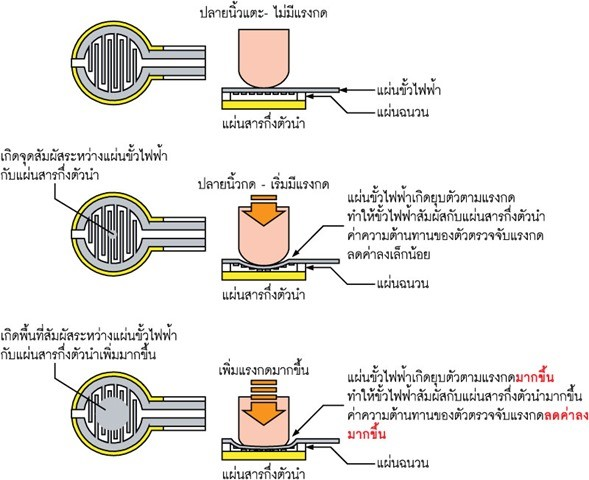
\includegraphics[width=0.5\textwidth]{chapter3/images/FSRfunction.jpg}
    \caption{การทำงานของตัวตรวจจับแรงกด FSR}
    \label{fig:FSRfunction}
\end{figure}

แนวคิดการออกแบบหลัก คือการออกแบบให้สามารถติดตั้งกับตัวหุ่นยนต์ได้เลย ไม่ต้องเชื่อมต่อสายไฟและสายส่งข้อมูลใหม่ โดยให้ใช้สายไฟไฟเลี้ยง 
และสายสัญญาณชุดเดียวกับตัวขับเคลื่อน Dynamixel Servo Mo-tor ซึ่งมีการติดต่อกันในลักษณะเป็นบัสแบบ RS-485 ดังนั้นแล้วผู้เขียนจึงเลือกที่จะทำโมดูลขึ้นมาใหม่ 1 โมดูล 
เพื่อที่ใช้ในการอ่านค่า Ground Contact Sensor ของหุ่นยนต์โดยเฉพาะ โดยมีการติดต่อรูปแบบบัส RS-485 ใช้ลักษณะการติดต่อสื่อสาร(Protocol) เดียวกับตัวขับเคลื่อน Dynamixel 
และมีการพัฒนาจาก Arduino ซึ่งให้สามารถอ่านค่าได้ทั้ง Analog และ Digital ได้ อีกทั้งรองรับการต่อ Sensor แบบ Force sensitive resistor จำนวน 4 ตัว.
\begin{figure}[!ht]
  \centering
  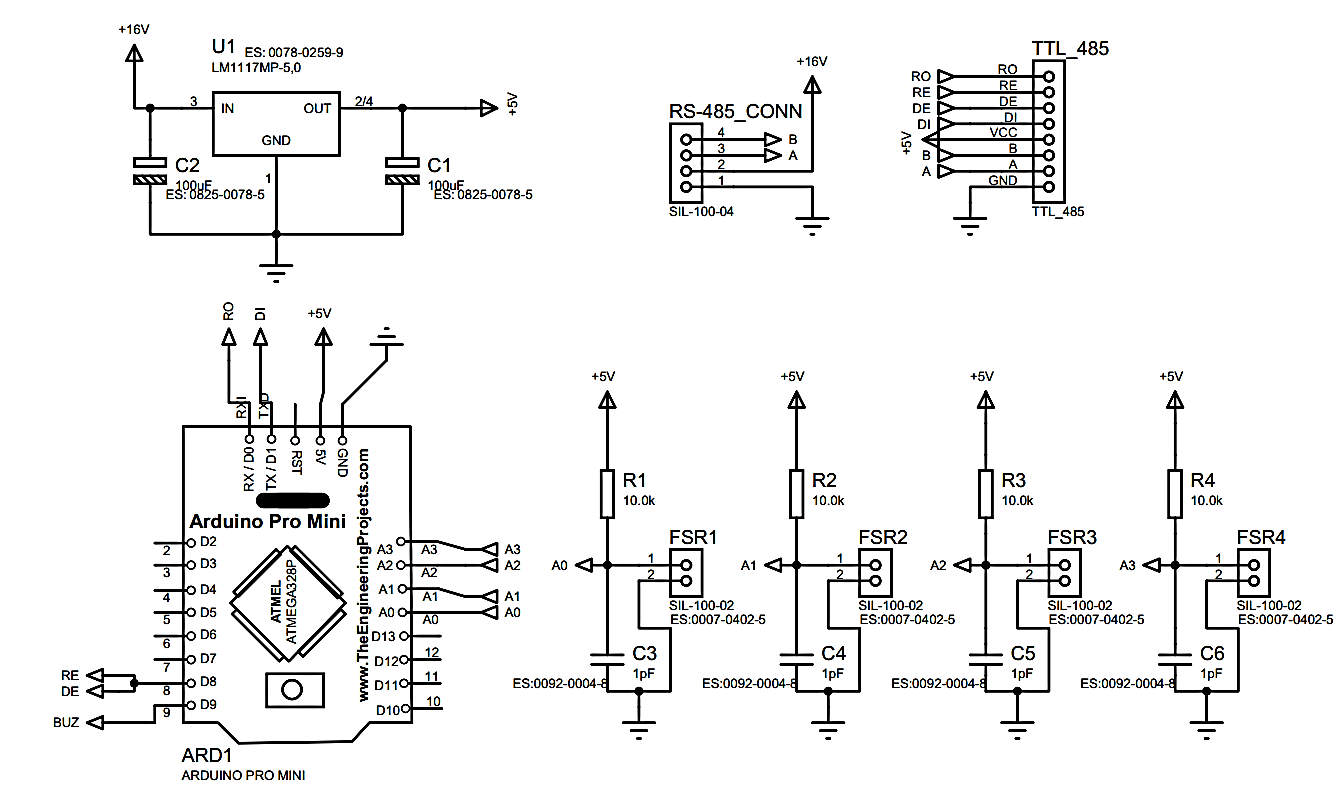
\includegraphics[width=0.8\textwidth]{chapter3/images/FSR_schematic.png}
  \caption{Schematic ของวงจร Ground Contact Sensor}
  \label{fig:FSR_schematic}
\end{figure}

\begin{figure}[!ht]
  \centering
  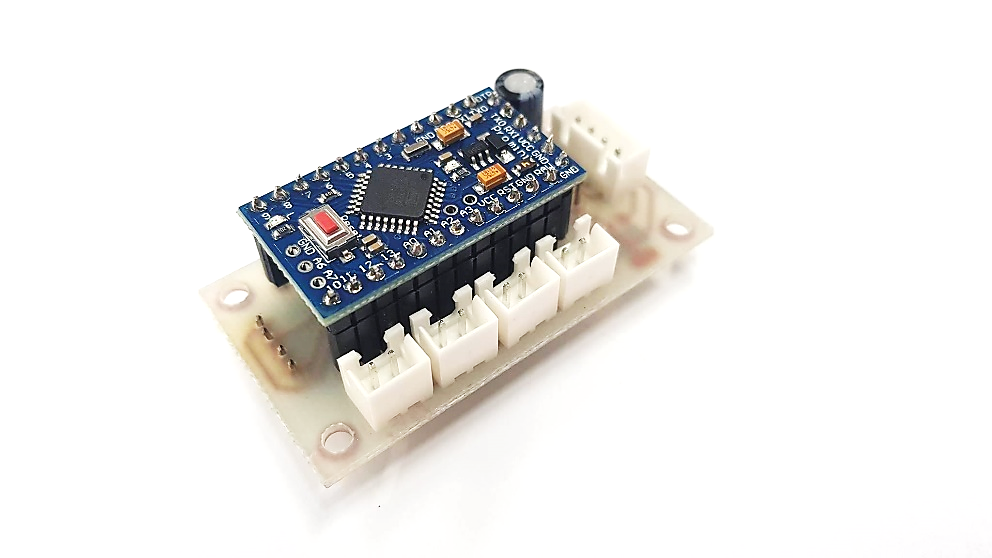
\includegraphics[width=0.8\textwidth]{chapter3/images/complete_FSR.png}
  \caption{แผงวงจร Ground Contact Sensor ที่ประกอบเสร็จแล้ว}
  \label{fig:complete_FSR}
\end{figure}

\clearpage
เซนเซอร์ที่เลือกใช้คือ Force Sensitive Resistor (FSR) เป็นเซนเซอร์ที่มีค่าความต้านทานภายในตัวเอง โดยเซนเซอร์นี้มีหลักการทำงานคือ 
ค่าความต้านทานทางไฟฟ้าของตัวเซนเซอร์จะเปลี่ยนแปลงเมื่อมีแรงเข้ามากระทำกับหน้าสัมผัส เมื่อมีแรงเข้ามากระทำมาก จะทำให้ค่าความต้านทานต่ำ 
หากไม่มีแรงเข้ามากระทำจะทำให้มีค่าความต้านทานสูง และเมื่อมีการนำเซนเซอร์นี้มาต่อกับตัวต้านทานที่มีค่าคงที่ ในรูปแบบของ Voltage Divider 
ดังรูปที่ \ref{fig:FSR_schematic} จะทำให้สามารถอ่านค่าแรงดันไฟฟ้าที่เปลี่ยนแปลงตามแรงที่เกิดขึ้นกับหน้าสัมผัสของเซนเซอร์ FSR ได้ 

\begin{figure}[!ht]
  \centering
  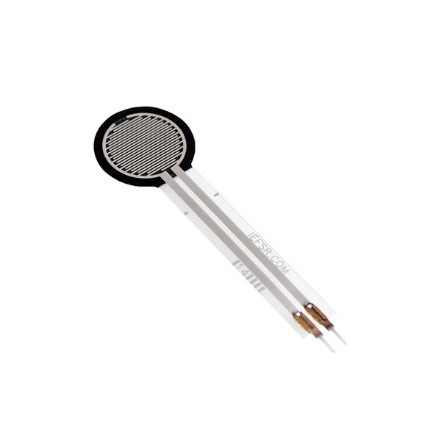
\includegraphics[width=0.3\textwidth]{chapter3/images/FSR.jpg}
  \caption{Force Sensitive Resistor (FSR) ขนาด 0.5 นิ้ว}
  \label{fig:FSR}
\end{figure}

ข้อดีของ FSR นั้นคือ เป็นเซนเซอร์ที่ถูกพัฒนาและออกแบบมาเพื่อใช้สำหรับการวัดแรงโดยตรง จึงทำให้ใช้งานได้ง่าย และสะดวก ในราคาที่ถูกกว่า 
เมื่อเทียบกับเซนเซอร์ Load cell ที่มีราคาสูงและการใช้งานจำเป็นที่จะต้องมีวงจรขยายสัญญาณที่ใช้ในการอ่านค่าการบิดของวัสดุจาก 
แต่ FSR นั้นก็มีข้อเสียเช่นกันคือ ความไม่ทนทานต่อการขีดข่วน เนื่องจากตัวเซนเซอร์ถูกทำมาจากฟิล์มพลาสติกบางๆ ซึ่งหากเกิดการขีดข่วนเกิดขึ้นแล้วอาจทำให้ฟิล์มฉีกขาดได้ 
หากฟิล์มขาดจะทำให้ค่าความต้านทานออกมาไม่เหมือนเดิม ดังนั้นทางผู้เขียนจึงเลือกที่จะออกแบบโครงครอบสำหรับเซนเซอร์ FSR เพื่อป้องกันจากการถูกขีดข่วนจากภายนอก







%%%%%%%%%%%%%%%%%%%%%%%%%%%%%%%%%%%%%%%%%%%%%%%%%%%%%%%%%%%%%%%%%%%%%%%%%%%%%%%
\clearpage
\subsection{การเชื่อมต่อตัวขับเคลื่อนและตัวรับรู้}
โครงสร้างของหุ่นยนต์ฮิวมานอยด์ UTHAIจะมีขาสองข้างทำให้เกิดองศาอิสระ 12 องศาอิสระ
จึงใช้ดิจิตอลเซอร์โวทั้งหมด 12 ตัว ดิจิตอลเซอร์โวทุกตัวเชื่อมต่อกันแบบสายโซ่เดซี่ (daisy chain) ดังรูปที่ \ref{fig:dynamixel_connect}
ข้างหนึ่งของมอเตอร์ตัวแรกเชื่อมต่อกับแบตเตอร์รี่ 12V และอีกข้างต่อกับ USB2RS485 เพื่อต่อไปยังตัวประมวลผลระดับสูง (Odroid)
และเซนเซอร์หน่วยวัดความเฉื่อย กับเซนเซอร์ตรวจจับหน้าสัมผัสที่พื้นเชื่อมต่อกับตัวประมวลผลระดับต่ำ (Nucleo F411RE)
ดังรูปที่ \ref{fig:odroid2dynamixel}
\begin{figure}[!ht]
    \centering
    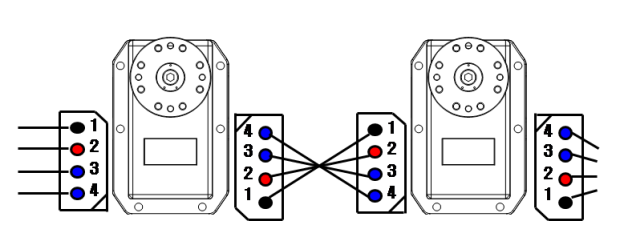
\includegraphics[width=0.7\textwidth]{chapter3/images/dynamixel_connect.png}
    \caption{การเชื่อมต่อกันระหว่างดิจิตอลเซอร์โว}
    \label{fig:dynamixel_connect}
\end{figure}
\begin{figure}[!ht]
    \centering
    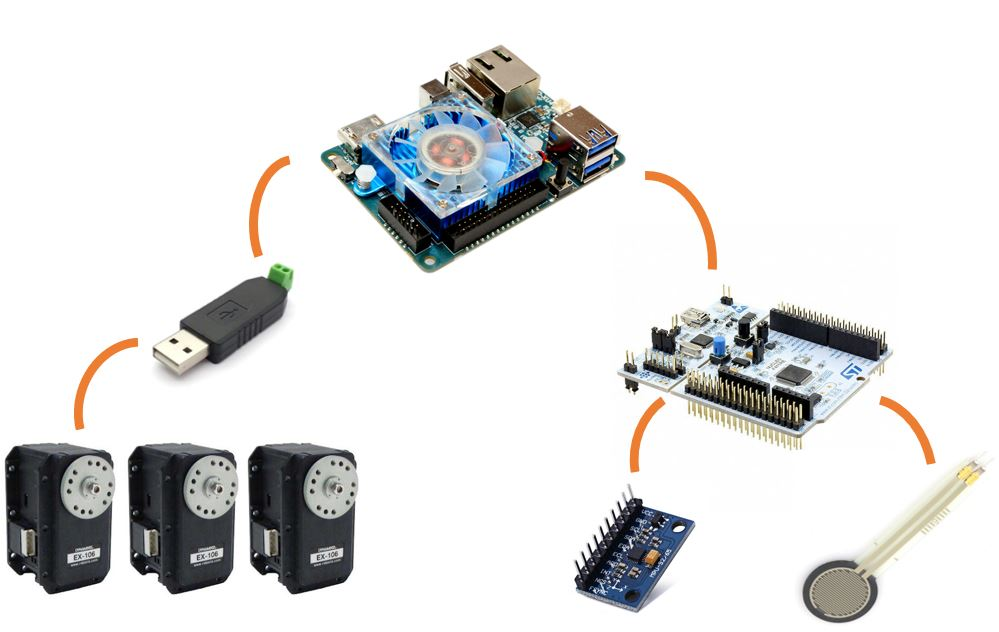
\includegraphics[width=0.9\textwidth]{chapter3/images/odroid2dynamixel.JPG}
    \caption{การเชื่อมต่อระหว่างตัวรับรู้ ตัวประมวลผล และตัวขับเคลื่อน}
    \label{fig:odroid2dynamixel}
\end{figure}


%%%%%%%%%%%%%%%%%%%%%%%%%%%%%%%%%%%%%%%%%%%%%%%%%%%%%%%%%%%%%%%%%%%%%%%%%%%%%%%
\clearpage
\subsection{การตั้งค่าดิจิตอลเซอร์โว}

\begin{wrapfigure}{l}{0.2\textwidth}
    
\includegraphics[width=0.9\linewidth]{chapter3/images/roboplus/roboplus.jpg} 
    \caption*{Roboplus 1.0}
\end{wrapfigure}

ก่อนที่จะเชื่อมต่อดิจิตอลเซอร์โวเข้ากับระบบประมวลผล จำเป็นที่จะต้องมีการตั้งค่า ID, Baudrate, Joint limited 
ของดิจิตอลเซอร์โว โดยการตั้งค่าพารามิเตอร์ของดิจิตอลเซอร์โวนั้น ผู้วิจัยจะใช้โปรแกรมที่มีชื่อว่า
Roboplus 1.0 ซึ่งเป็นเครื่องมือจากบริษัท Robotis ที่จำหน่ายดิจิตอลเซอร์โวนี้ โดยจะช่วยให้สามารถติดต่อกับดิจิตอลเซอร์โว
ตั้งค่าพารามิเตอร์ได้ แต่โปรแกรม Roboplus 1.0 นี้ใช้ได้เฉพาะใน Windows OS เท่านั้น ซึ่งสามารถดาวน์โหลดโปรแกรมได้จากหน้าเว็บไซต์ Robotis\footnote{http://www.robotis.us/roboplus1/}
เมื่อดาวน์โหลดโปรแกรมและติดตั้งเรียบร้อยแล้ว ให้เชื่อมต่อดิจิตอลเซอร์โวกับคอมพิวเตอร์ด้วย USB2RS485
และตั้งค่าพารามิเตอร์โดยทำตามขั้นตอน ดังรูปต่อไปนี้
\begin{figure}[!ht]
    \centering
    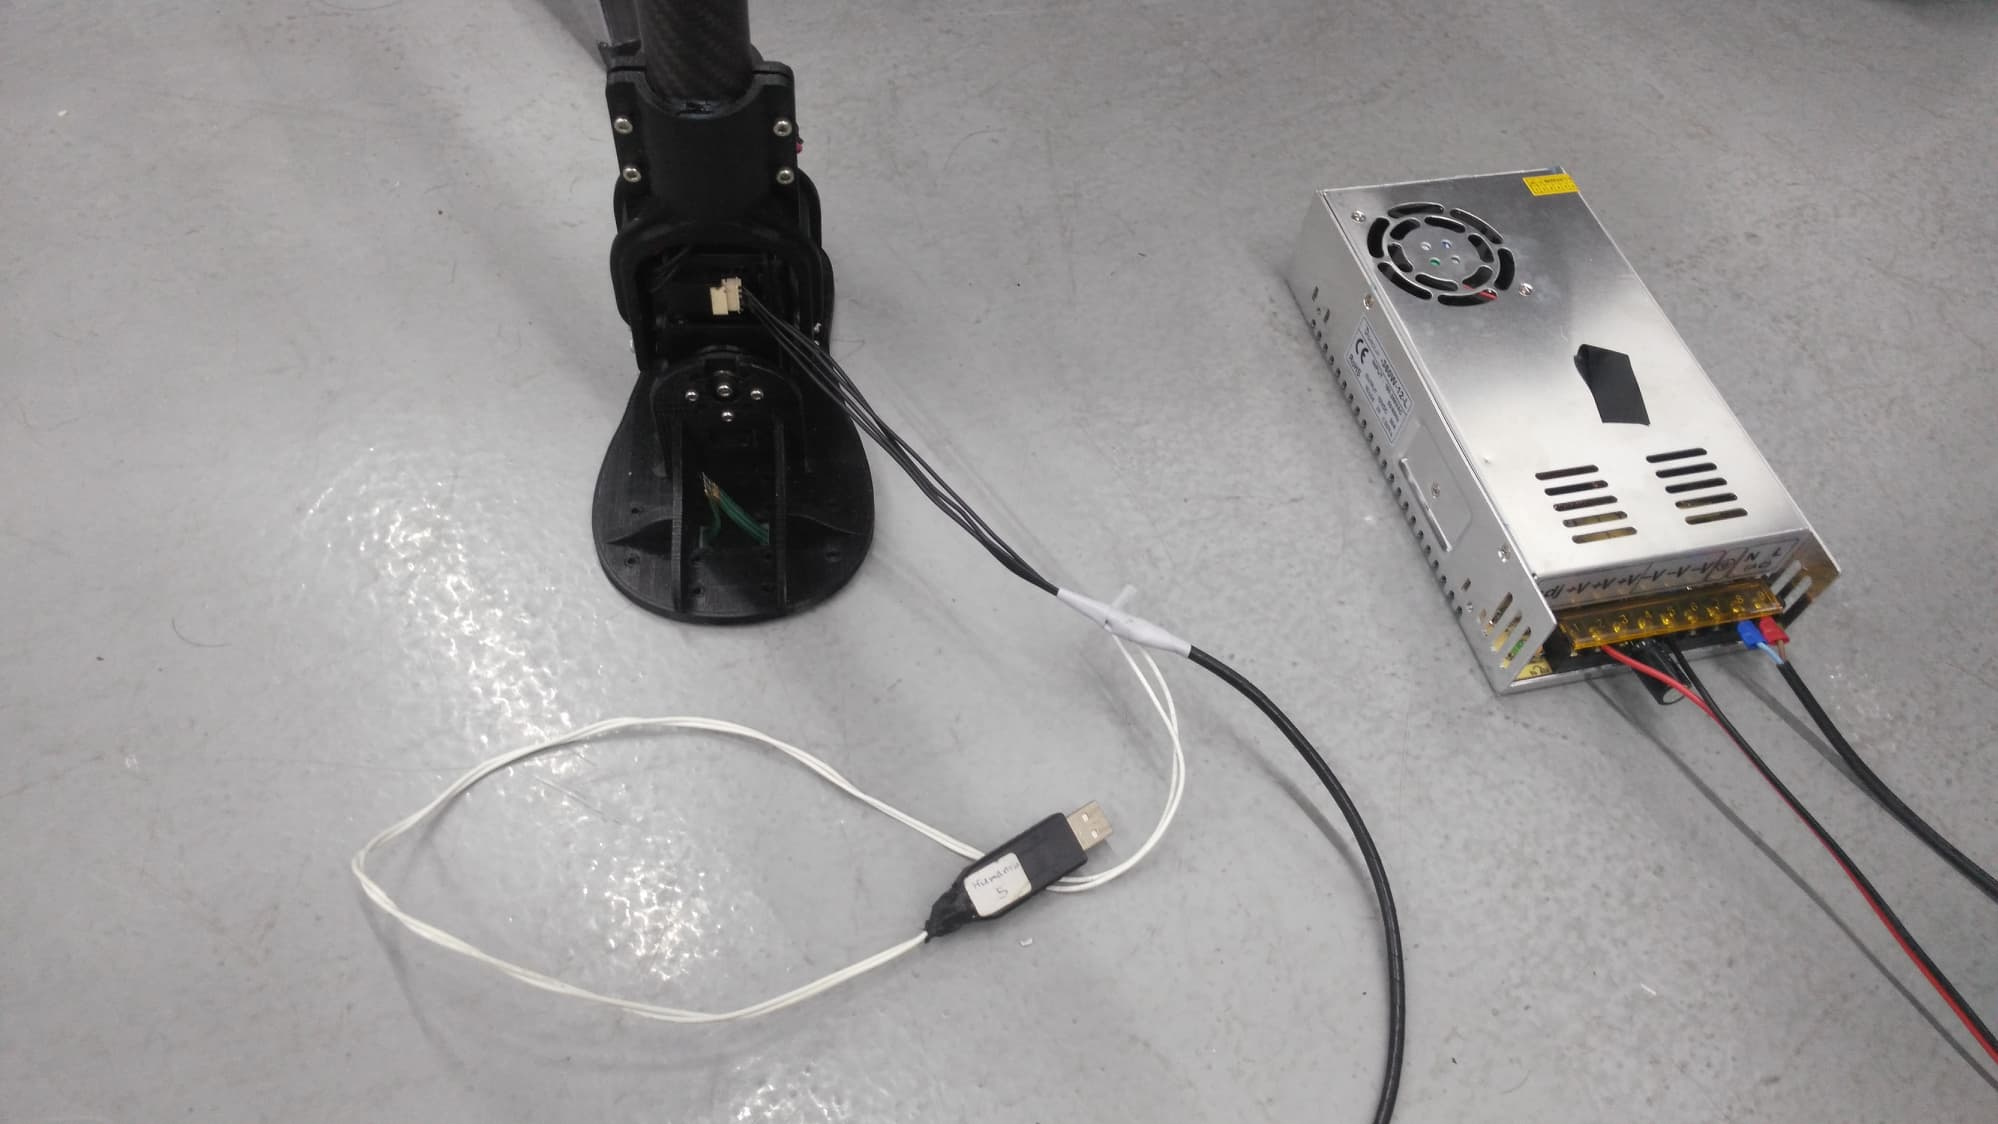
\includegraphics[width=\textwidth]{chapter3/images/roboplus/roboplus0.jpg}
    \caption*{เชื่อมต่อดิจิตอลเซอร์โวเข้ากับคอมพิวเตอร์ด้วย USB2RS485}
\end{figure}
\begin{figure}[!ht]
    \centering
    
\includegraphics[width=0.25\textwidth]{chapter3/images/roboplus/roboplus1.PNG}
    \caption*{เปิดโปรแกรม Roboplus 1.0}
\end{figure}
\begin{figure}[!ht]
    \centering
    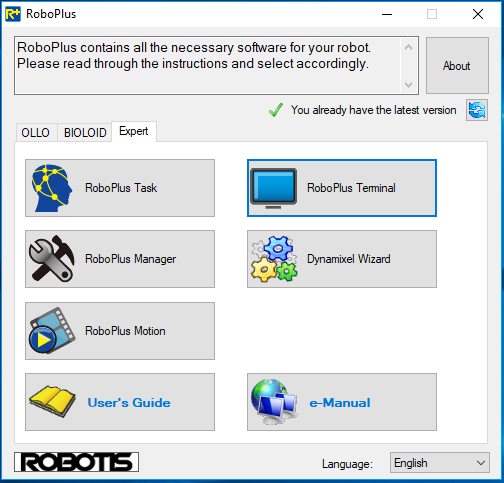
\includegraphics[width=0.55\textwidth]{chapter3/images/roboplus/roboplus2.PNG}
    \caption*{กดเข้าไปที่ Dynamixel Wizard}
\end{figure}
\begin{figure}[!ht]
    \centering
    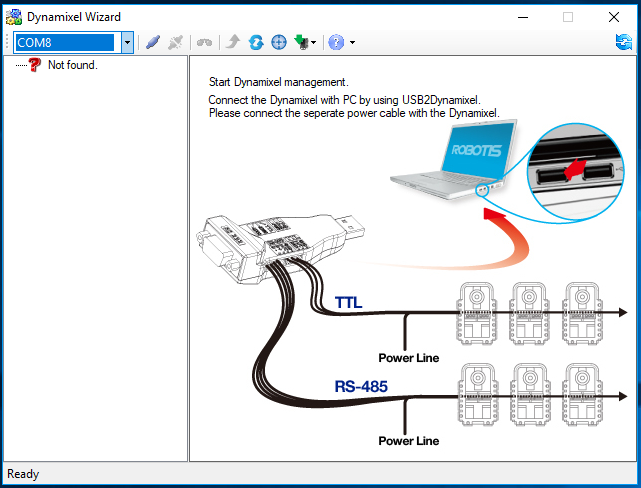
\includegraphics[width=0.55\textwidth]{chapter3/images/roboplus/roboplus3.PNG}
    \caption*{เลือก COM Port ให้ตรงกับ USB2RS485 จากนั้นกด Connect}
\end{figure}
\begin{figure}[!ht]
    \centering
    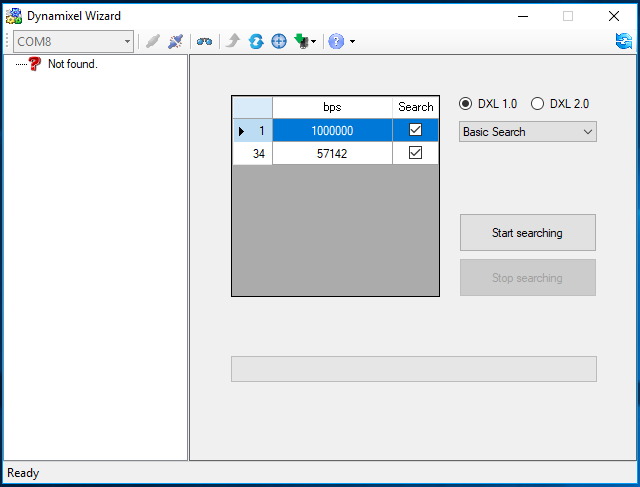
\includegraphics[width=0.55\textwidth]{chapter3/images/roboplus/roboplus4.PNG}
    \caption*{กดเลือกที่ช่อง 1Mbps แล้วกด Start searching}
\end{figure}
\begin{figure}[!ht]
    \centering
    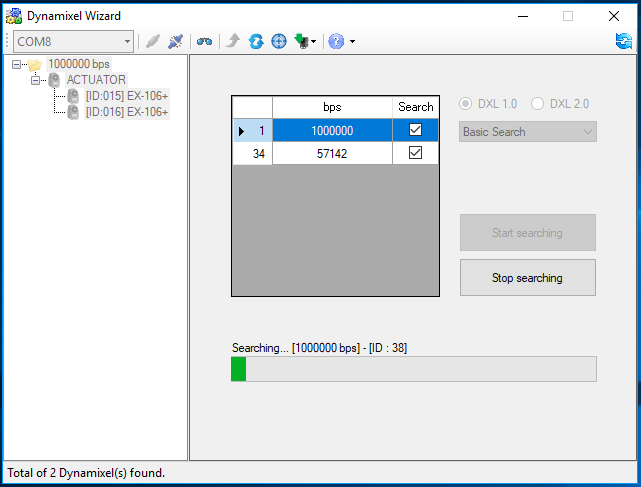
\includegraphics[width=0.55\textwidth]{chapter3/images/roboplus/roboplus5.PNG}
    \caption*{เมื่อเห็นทางด้านซ้ายมือโผล่ ID มอเตอร์ขึ้นมา หากขึ้นแล้วก็สามารถกด Stop Searching ได้}
\end{figure}
\begin{figure}[!ht]
    \centering
    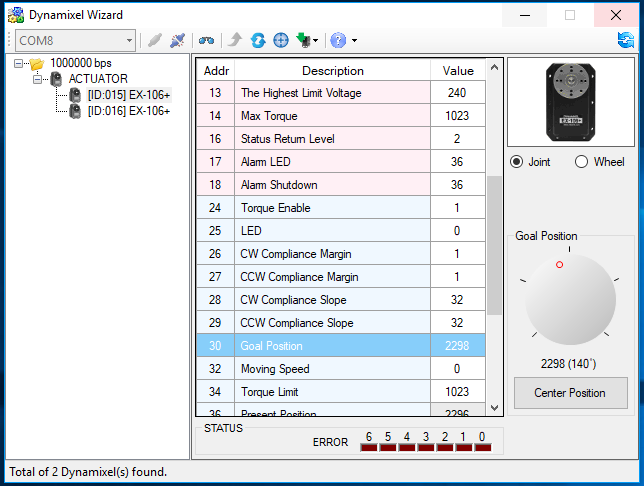
\includegraphics[width=0.55\textwidth]{chapter3/images/roboplus/roboplus6.PNG}
    \caption*{ทดสอบสั่งการมอเตอร์ที่ Addr 30 Goal position ว่าทิศทางถูกต้องหรือไม่}
\end{figure}
\begin{figure}[!ht]
    \centering
    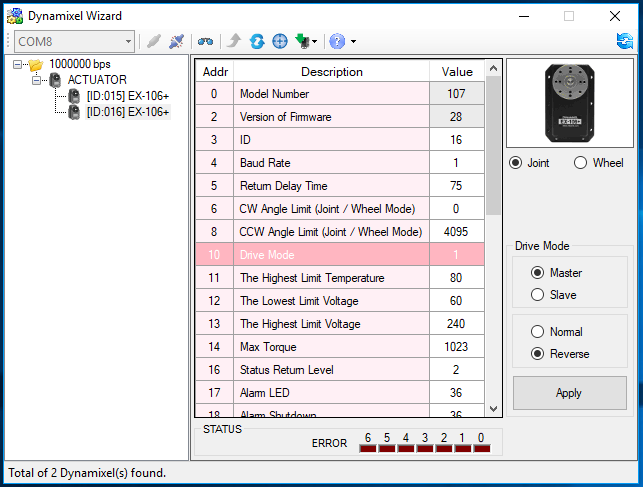
\includegraphics[width=0.55\textwidth]{chapter3/images/roboplus/roboplus7.PNG}
    \caption*{ถ้าทิศทางไม่ถูกต้องสามารถที่จะปรับได้ที่ Addr 10 Drive mode}
\end{figure}

%%%%%%%%%%%%%%%%%%%%%%%%%%%%%%%%%%%%%%%%%%%%%%%%%%%%%%%%%%%%%%%%%%%%%%%%%%%%%%%
\clearpage
\subsection{การเชื่อมต่อบอร์ดประมวลผล}
การเชื่อมต่อระหว่างบอร์ดประมวลผลระดับล่างกับบอร์ดประมวลผลระดับสูง โดยจะเชื่อมต่อกันผ่านสาย USB
และส่งข้อมูลหากันผ่านซีเรียลโดยใช้ rosserial นอกจากจะมีบอร์ดประมวลผลแล้วยังมีบอร์ดที่เอาไว้ใช้สำหรับควบคุม
ดิจิตอลเซอร์โวเพื่อเผื่อเอาไว้สำหรับเปลี่ยนให้ ตัวประมวลผลควบคุมระดับล่างเป็นตัวสั่งการมอเตอร์
ดัวรูปที่ \ref{fig:uthai_controller}

\begin{figure}[!ht]
    \centering
    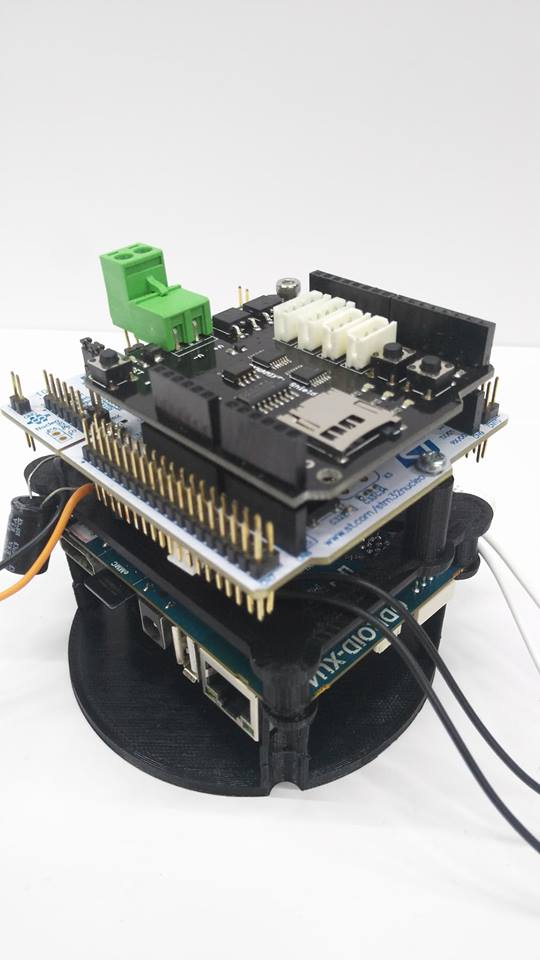
\includegraphics[width=0.4\textwidth]{chapter3/images/uthai_controller.jpg}
    \caption{การเชื่อมต่อกันระหว่างตัวประมวลผล}
    \label{fig:uthai_controller}
\end{figure}






\clearpage
\section{การออกแบบโปรแกรมด้วย ROS}
\subsection{Modelling}
หลังจากที่เราได้ออกแบบและโมเดลหุ่นยนต์ของเราขึ้นมาที่ใช้ CAD tools ต่างๆ เช่น AutoCAD, SolidWorks, Blender
หรืออื่นๆ ก็เพื่อที่จะนำมาใช้ในการทำ Simulation การที่เราทำ Simulation นั้นก็จะสามารถมองเห็นหุ่นยนต์
และเห็นการทำงานของหุ่นยนต์เราก่อนที่เราจะสร้างมันขึ้นมาจริงๆ หุ่นยนต์จำลองที่เราสร้างขึ้นมานั้นควรที่จะมีลักษณะให้ใกล้เคียงกับของจริงมากที่สุด
ไม่ว่าจะเป็นรูปร่าง รูปทรง น้ำหนักต่างๆ 

\subsubsection{ROS packages for robot modelling}
ROS นั้นได้ให้เครื่องมือที่ช่วยให้เราสามารถสร้าง 3D robot models ได้
ใน ROS มี meta package ที่ชื่อว่า robot\_model ซึ่งข้างในมี package ต่างๆที่ใช้สำหรับสร้าง 3D robot models
        
\paragraph*{urdf}
เป็น 1 ในหลายๆ package ที่อยู่ใน robot\_model, urdf เป็น xml ไฟล์ที่เอาไว้ใช้บอกลักษณะของหุ่นยนต์ ย่อมาจาก Unified Robot Description Format(URDF)
เราสามารถระบุ robot model, sensors และ working environment โดยใช้ URDF การบอกนั้นจะสามารถบอกเป็นเหมือน tree structure ของ link ต่างๆในตัวหุ่นยนต์ สามารถบอก rigid link เชื่อมต่อกันผ่าน joints แต่ถ้าเป็น flexible link จะไม่สามารถบอกได้โดยใช้ urdf

\subparagraph*{joint\_state\_publisher}
เครื่องมือนี้มีประโยชน์มากในการ model robot URDF เพราะมันสามารถหา joints ทุก joint ที่ไม่ใช่ fixed joints มาแสดงเป็น GUI sliders ทำให้เราสามารถเลื่อนๆหมุนๆไปมาได้ อีกทั้งยังสามารถใช้งานร่วมกับ visualize RViz

\subparagraph*{robot\_state\_publisher}
เป็นเครื่องมือที่ใช้ในการ publish 3d pose ของ link ต่างๆใน urdf การ ยublish นั้นจะใช้ ROS tf(transform) ROStf คือการหาความสัมพันธ์ระหว่าง frame ของหุ่นยนต์

\subparagraph*{xacro}
ย่อมาจาก XML Macros หรือเราสามารถเรียกอีกอย่างว่า URDF plus add-ons. ซึ่งการทำงานเหมือนกับ urdf แต่ทำให้ไฟล์ urdf สั้นกว่า อ่านง่ายกว่า และสามารถใช้เพื่อทำให้สร้างหุ่นยนต์ที่มีความซับซ้อนง่ายขึ้น เราสามารถแปลงไฟล์ xacro เป็น urdf ได้

\subsubsection{URDF}
ในส่วนนี้จะเป็นการอธิบายระบบทางกลของหุ่นยนต์ฮิวมานอยด์เป็นไฟล์ที่ใช้ร่วมกับ ROS ได้ เพื่อที่จะสามารถนำไปใช้กับ Simulation ในอนาคตได้
ในการอธิบายระบบทางกลนั้นผู้วิจัยได้ใช้ไฟล์ URDF (Universal Robotics Description Format) ซึ่งใช้ภาษาการเขียนเป็น XML ในการบอกส่วนประกอบแต่ละส่วนของหุ่นยนต์

\subsubsection*{Link}
ในไฟล์ URDF แต่ละชิ้นส่วนของหุ่นยนต์เราจะเรียกว่า link แล้วใน link จะประกอบไปด้วยส่วนย่อยๆ
3 ส่วนคือ <inertia> ที่เอาไว้บอกถึงค่าตัวแปรทางฟิสิกส์, <visual> ที่เอาไว้แสดงผลให้เราเห็น, 
<collision> ที่เอาไว้ตรวจสอบว่าหุ่นยนต์มีการชนกันกับสิ่งแวดล้อมไหม ดังรูปที่ \ref{fig:urdf_link_code}

\clearpage
\begin{figure}[ht]
\begin{Verbatim}[fontsize=\small]
<link name="my_link">
    <inertia>
        <origin xyz="0 0 0.5" rpy="0 0 0"/>
        <mass value="1"/>
        <inertia ixx="100" ixy="0" ixz="0" iyy="100" iyz="0" izz="100"/>
    </inertia>
    <visual>
        <origin xyz="0 0 0" rpy="0 0 0"/>
        <geometry>
            <box size="1 1 1" />
        </geometry>
        <material name="Cyan">
            <color rgba="0 1.0 1.0 1.0"/>
        </material>
    </visual>
    <collision>
        <origin xyz="0 0 0" rpy="0 0 0"/>
        <geometry>
            <cylinder radius="1" length="0.5"/>
        </geometry>
    </collision>
</link>
\end{Verbatim}
\caption{ตัวอย่าง link ใน urdf}
\label{fig:urdf_link_code}
\end{figure}

ยังมี tags อีกหลายตัวที่ใช่ในการอธิบายแต่ละชิ้นส่วนของหุ่นยนต์ แต่ตัวอย่างเป็นเพียงแค่ส่วนหนึ่งเท่านั้น
ในความเป็นจริงแล้วเราจะเขียน tags ต่างๆก็ตามที่เราต้องการ โดยใน URDF ไฟล์นั้นจะเอาไว้เก็บข้อมูลลักษณะเฉพาะของหุ่นยนต์เอาไว้
และยังสามารถใช้กับซอฟแวร์ตัวอื่นๆอีกได้

\begin{figure}[ht]
	\centering
	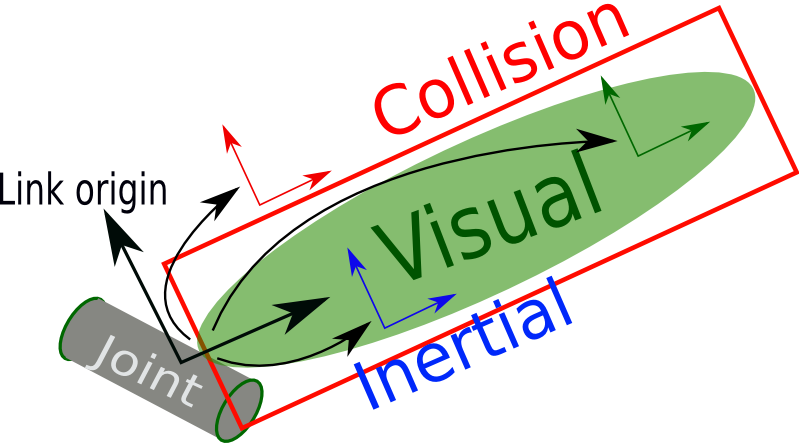
\includegraphics[width=0.60\textwidth]{chapter3/images/urdf_link.png}
	\caption{การอธิบาย link ใน URDF ไฟล์}
	\label{fig:urdf_link}
\end{figure}

\clearpage
\subsubsection*{Joint}
อีกส่วนที่สำคัญสำหรับการสร้างไฟล์หุ่นยนต์ด้วย URDF ก็คือ Joint tag โดย tag นี้จะอธิบายถึงความสัมพันธ์ระหว่างก้านต่อสองอัน
ส่วนนี้ไม่ได้มีเพียงแค่ทำข้อต่อให้เป็นแบบหมุนได้อย่างเดียว ยังมี Fix, Revolution, Linear และ Planar นอกเหนือจากนี้
เรายังสามารถที่จะเพิ่มองศาสูงสุดต่ำสุดของข้อต่อ รวมไปถึง dynamic properties ต่างๆ ตามที่เห็นดังรูปที่ \ref{fig:urdf_joint_code}
\begin{figure}[ht]
\begin{Verbatim}[fontsize=\small]
<joint name="my_joint" type="floating">
	<origin xyz="0 0 1" rpy="0 0 3.1416"/>
	<parent link="link1"/>
	<child link="link2"/>
	<calibration rising="0.0"/>
	<dynamics damping="0.0" friction="0.0"/>
	<limit effort="30" velocity="1.0" lower="-2.2" upper="0.7"/>
	<safety_controller k_velocity="10" k_position="15" 
	soft_lower_limit="-2.0" soft_upper_limit="0.5"/>
</joint>
\end{Verbatim}
\caption{ตัวอย่าง joint ใน urdf}
	\label{fig:urdf_joint_code}
\end{figure}

เมื่อเรานำ Joint และ Link มารวมกันเราจะต้องพิจารณาว่ามีวางรูปแบบเป็นไปตามรูปที่ \ref{fig:urdf_joint}
โดยจะมีระยะระหว่างแกนของแต่ละข้อต่อกับก้านต่อ ชิ้นส่วนแรกของการสร้างไฟล์ URDF จะมีชื่อว่า base\_link
และเฟรม origin จะเป็นเฟรมอ้างอิง เมื่อเราต่อ Joint เข้ากับ Link จะเรียกก้านต่อที่เอามาติดว่า parent
โดยเฟรม origin ของข้อต่อจะอยู่จุดเดียวกับเฟรม origin ของก้านต่อ ในสถานะเดียวกันก้านต่อที่นำมาต่อจากข้อต่อ
เราจะเรียกว่า child และเฟรม origin ของก้านต่อ child จะอยู่ที่จุดเดียวกับเฟรม origin ของข้อต่อ

\begin{figure}[h]
	\centering
	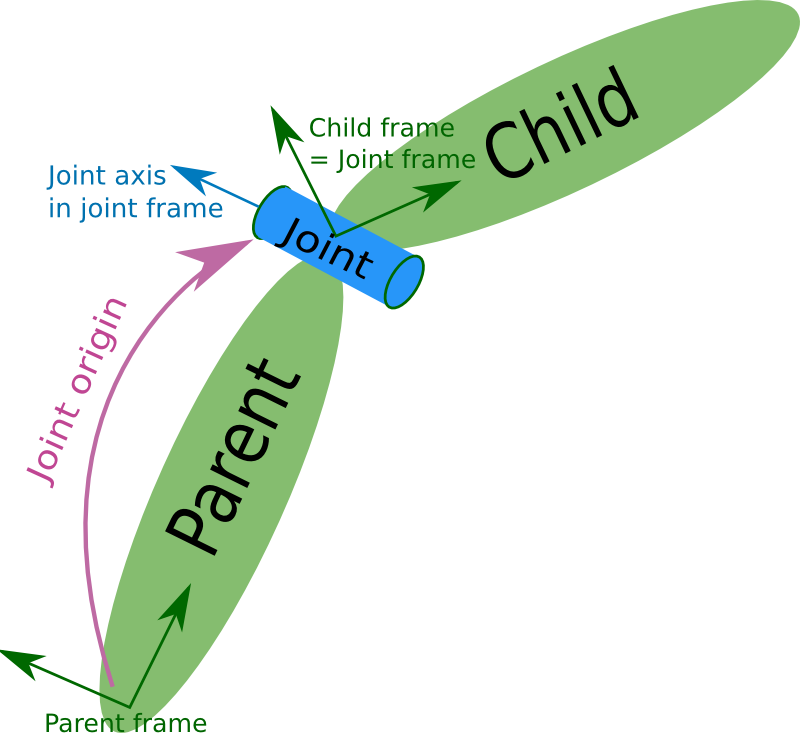
\includegraphics[width=0.55\textwidth]{chapter3/images/urdf_joint.png}
	\caption{การอธิบาย Joint ใน URDF ไฟล์}
	\label{fig:urdf_joint}
\end{figure}

%%%%%%%%%%%%%%%%%%%%%%%%%%%%%%%%%%%%%%%%%%%%%%%%%%%%%%%%%%%%%%%%%%%%%%%%%%%%%%%
\clearpage
\subsection{กำหนดพิกัดเฟรมให้กับหุ่นยนต์ฮิวมานอยด์}
การกำหนดเฟรมให้กับหุ่นยนต์ฮิวมานอยด์นั้นเราจะใช้หลักตามของ ROS Enhancement Proposals (REPs) ซึ่งจะทำให้เราสามารถใช้เครื่องมือต่างๆ ที่มีคนสร้างขึ้นมาใช้งานได้ง่าย และช่วยทำให้เกิดความเข้าใจได้ง่าย

\subsubsection*{base\_link}
เป็นเฟรมที่ติดอยู่กับฐานของหุ่นยนต์ โดยจะติดตำแหน่งหรือมุมเอียงใดก็ได้ ปกติแล้วจะติดที่สะโพกของหุ่นยนต์

\subsubsection*{base\_footprint}
เป็นเฟรมที่เอาไว้แสดงว่าหุ่นยนต์อยู่ตรงไหนบนพื้นโลก โดยปกติแล้วจะมีระดับอยู่ที่จุดต่ำสุดของฝ่าเท้า z = min(l\_sole\_z,r\_sole\_z)
โดย l\_sole\_z และ r\_sole\_z คือความสูงของฝ่าเท้าซ้ายและขวา base\_footprint เหมือน 2D planar
ที่บอกตำแหน่งของฮิวมานอยด์ระหว่างที่กำลังเดินหรือทำอย่างอื่นอยู่

\subsubsection*{l\_wrist, r\_wrist}
เป็นเฟรมที่บอกตำแหน่งและมุมเอียงของแขนซ้ายและขวาแต่ไม่ได้คำนึงถึงการติดตั้งอุปกรณ์ใดๆเข้าไป

\subsubsection*{l\_gripper, r\_gripper}
เป็นเฟรมที่บอกตำแหน่งและมุมเอียงของที่ปลายแขน (End effector) ถ้ามือจับอุปกรณ์อยู่ เฟรมนี้ก็จะไปอยู่ในตำแหน่งของอุปกรณ์นั้นๆ

\subsubsection*{l\_ankle, r\_ankle}
เป็นเฟรมที่บอกตำแหน่งและมุมเอียงของขาซ้ายและขวาโดยไม่ได้คำนึงว่าจุดรับน้ำหนักของตัวอยู่ที่ไหน

\subsubsection*{l\_sole, r\_sole}
เป็นเฟรมที่บอกตำแหน่งและมุมเอียงของขาซ้ายและขวาที่รองรับน้ำหนักตัวอยู่ โดยจะบอกการ projection ของ X,Y ใน 2D plane ที่สัมผัสพื้นและ Z จะอยู่ระดับเดียวกับพื้นสัมผัส

\subsubsection*{l\_toe, r\_toe}
เป็นเฟรมที่บอกตำแหน่งและมุมเอียงของปลายเท้าซ้ายและขวา โดยอยู่บนพื้นผิวที่สัมผัสอยู่

\subsubsection*{gaze}
เป็นเฟรมที่บอกตำแหน่งและมุมเอียงของหัว โดยการเอียงนั้นจะบอกทิศทางของหัวโดยไม่ได้สนใจเซนเซอร์ว่าจะติดตั้งอย่างไร

\subsubsection*{torso}
เป็นเฟรมที่ติดอยู่กับลำตัวช่วงล่างของหุ่นยนต์โดยจะเป็นตัวที่เชื่อม ขา แขน ตัว หัว เข้าเอาไว้ด้วยกัน
%%%%%%%%%%%%%%%%%%%%%%%%%%%%%%%%%%%%%%%%%%%%%%%%%%%%%%%%%%%%%%%%%%%%%%%%%%%%%%%


\clearpage
\subsection{Box model}

\clearpage
\subsection{Dynamic properties}
ข้อมูล 
\begin{figure}[h!]
	\centering
	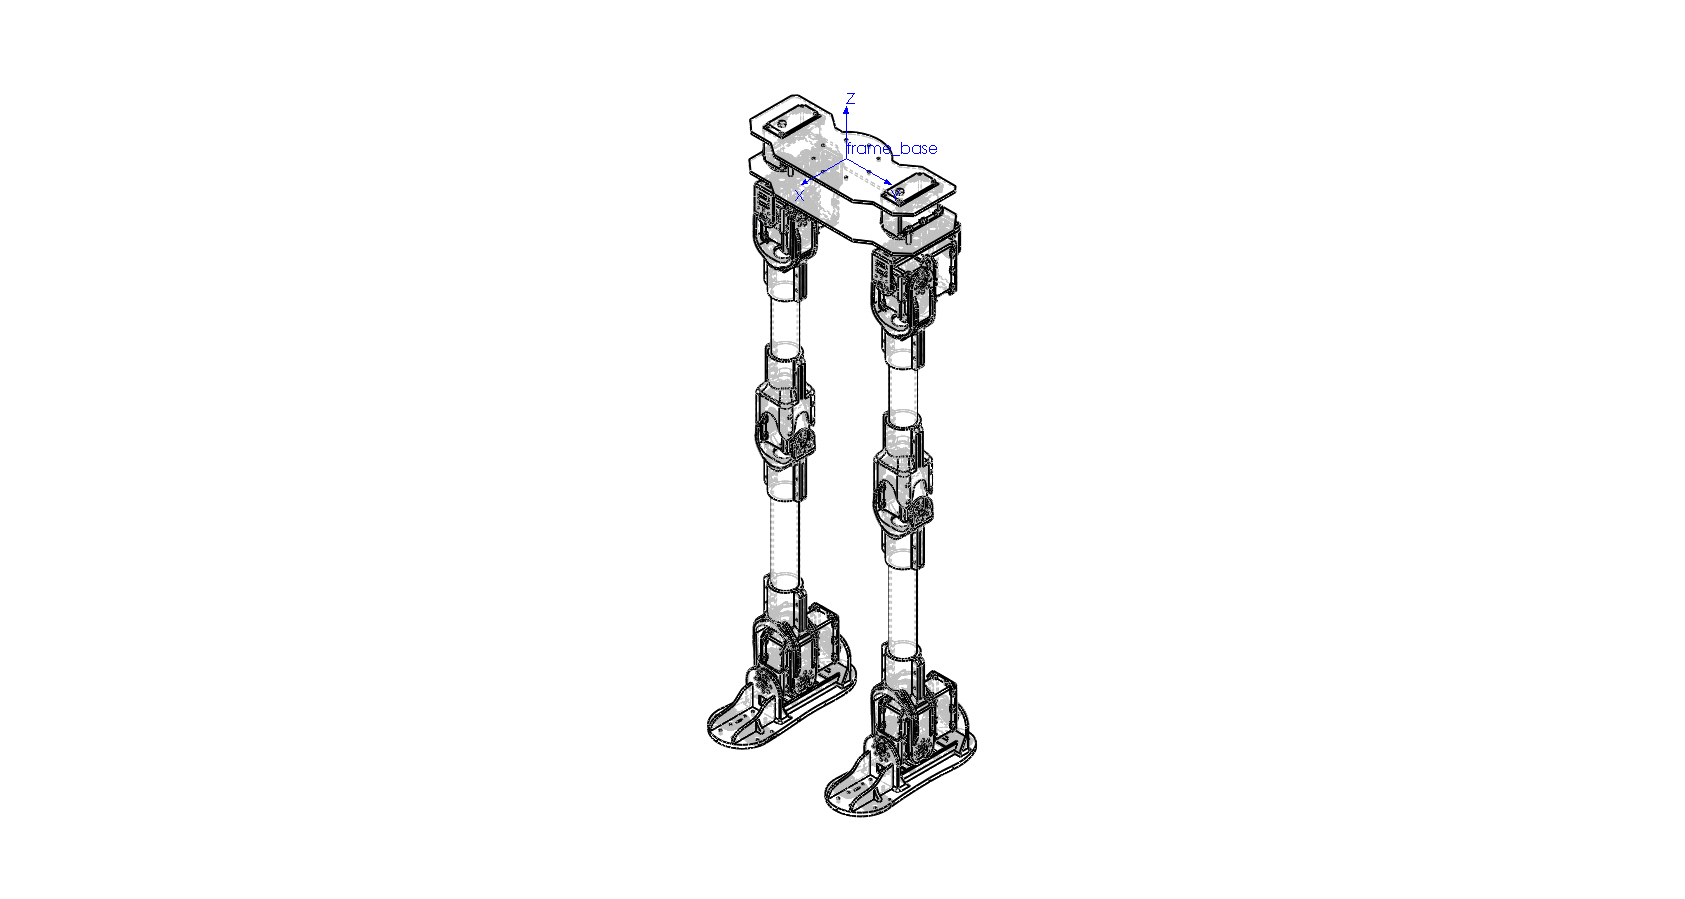
\includegraphics[width=\textwidth]{chapter3/images/uthai_dynamic_all.jpeg}
	\caption{ภาพแสดงช่วงล่างหุ่นยนต์ฮิวมานอยด์}
	\label{fig:uthai_dynamic_all}
\end{figure}
\begin{table}[h!]
	\centering
	\begin{tabular}{| c | c |}
		\hline
		Link & All Link\\
		\hline
		Mass (kg) & 3.31477475 \\
		CoM X (m) & -0.00855772 \\
		CoM Y (m) & 0.00000000 \\
		Inertia Ixx & 0.28641029 \\
		Inertia Ixy & -0.00000302 \\
		Inertia Ixz & -0.00048106 \\
		Inertia Iyy & 0.26207601 \\
		Inertia Iyz & -0.00061103 \\
		Inertia Izz & 0.02925799 \\
		\hline
	\end{tabular}
	\caption{Message Geometry Point}
	\label{tab:geometry_point}
\end{table}

%%%%%%%%%%%%%%%%%%%%%%%%%%%%%%%%%%%%%%%%%%%%%%%%%%%%%%%%%%%%%%%%%%%%%%%%%%%%%%%
%%%%%%%%%%%%%%%%%%%%%%%%%%%%%%%%%%%%%%%%%%%%%%%%%%%%%%%%%%%%%%%%%%%%%%%%%%%%%%%
\clearpage
\subsection{โครงสร้างการติดต่อสื่อสารระหว่าง Node ใน ROS}
การติดต่อสื่อสารกันภายใน ROS นั้นจะใช้การส่ง message หากัน ซึ่ง message แต่ละตัวก็จะใช้ในงานที่ต่างกัน
ตามระบบที่ต้องการส่ง จากรูปที่ \ref{fig:uthai_ros_node} เป็นโครงสร้างการส่งข้อมูลหากันของหุ่นยนต์ฮิวมานอยด์
ที่ผู้วิจัยได้ออกแบบไว้ โดยเริ่มจากผู้ใช้งานส่งตำแหน่งที่หุ่นยนต์จะต้องเดินไปไปยัง Node ที่ทำการคำนวณและสร้างตำแหน่งการวางเท้าของหุ่นยนต์
แล้วหลังจากนั้นจะส่งข้อมูลออกไปเป็น Path เส้นทางไปยัง Node ที่ทำการค้นหาตำแหน่งของ com, zmp ของหุ่นยนต์
เพื่อทำการควบคุมและสั่งการหุ่นยนต์ต่อไป

\begin{figure}[h!]
	\centering
	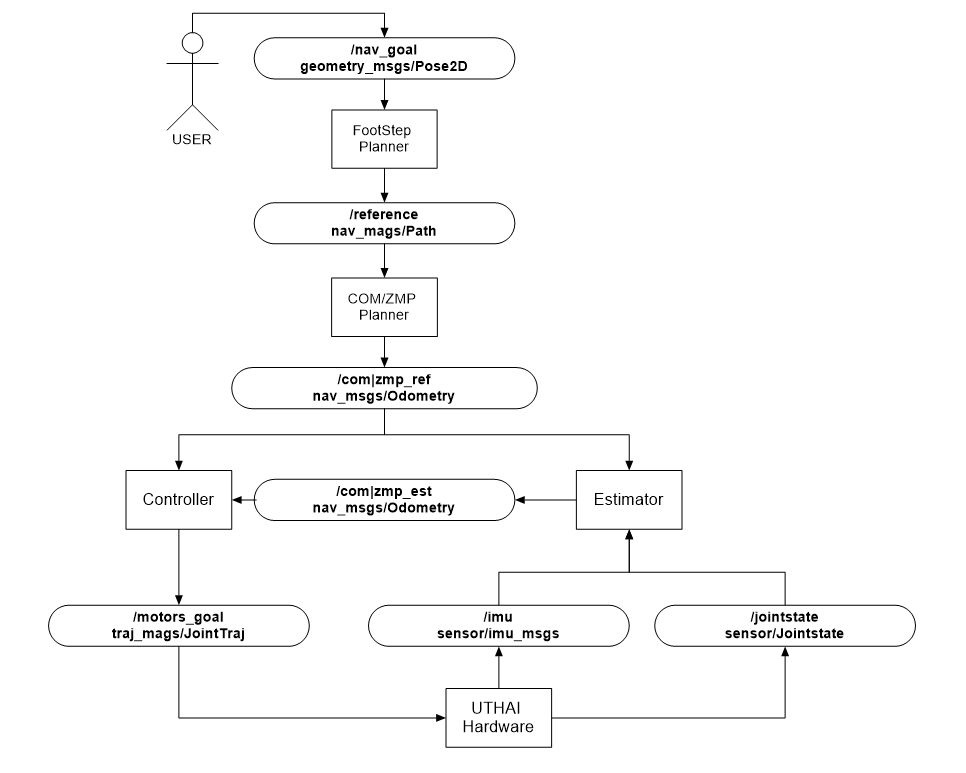
\includegraphics[width=\textwidth]{chapter3/images/uthai_ros_node.png}
	\caption{การติดต่อสื่อสารระหว่าง Node}
	\label{fig:uthai_ros_node}
\end{figure}

\subsubsection*{การบอกตำแหน่งและมุมเอียง}
การบอกตำแหน่งใน 3 มิติ Point คือการบอก $x$, $y$, $z$ และการบอกมุมเอียงจะใช้ Quaternion
ในการบอกโดยใช้ตัวแปรสี่ตัว คือ $x$,$y$,$z$,$w$ หากนำทั้งสองมารวมกันเราจะเรียกว่า Pose
\begin{table}[h!]
	\centering
	\begin{tabular}{| c | c |}
		\hline
		\multicolumn{2}{|c|}{geometry\_msgs/Point}\\
		\hline
		float64 & x \\
		float64 & y \\
		float64 & z \\
		\hline
	\end{tabular}
	\caption{Message Geometry Point}
	\label{tab:geometry_point}
\end{table}
\begin{table}[h!]
	\centering
	\begin{tabular}{| c | c |}
		\hline
		\multicolumn{2}{|c|}{geometry\_msgs/Quaternion}\\
		\hline
		float64 & x \\
		float64 & y \\
		float64 & z \\
		float64 & w \\
		\hline
	\end{tabular}
	\caption{Message Geometry Quaternion}
	\label{tab:geometry_quaternion}
\end{table}
\begin{table}[h!]
	\centering
	\begin{tabular}{| c | c |}
		\hline
		\multicolumn{2}{|c|}{geometry\_msgs/Pose}\\
		\hline
		geometry\_msgs/Point & position \\
		geometry\_msgs/Quaternion & orientation \\
		\hline
	\end{tabular}
	\caption{Message Geometry Pose}
	\label{tab:geometry_pose}
\end{table}

\subsubsection*{การบอกความเร็วเชิงเส้นและเชิงมุม}
การบอกความเร็วเชิงเส้นใน 3 มิติ คือการบอกความเร็วตามแนวแกน $x$, $y$, $z$ และการบอกความเร็วเชิงมุม
คือการบอกความเร็วการหมุนรอบแกน $x$,$y$,$z$ หากนำทั้งสองมารวมกันเราจะเรียกว่า Twist
\begin{table}[h!]
	\centering
	\begin{tabular}{| c | c |}
		\hline
		\multicolumn{2}{|c|}{geometry\_msgs/Vector3}\\
		\hline
		float64 & x \\
		float64 & y \\
		float64 & z \\
		\hline
	\end{tabular}
	\caption{Message Geometry Vector3}
	\label{tab:geometry_vector3}
\end{table}
\begin{table}[h!]
	\centering
	\begin{tabular}{| c | c |}
		\hline
		\multicolumn{2}{|c|}{geometry\_msgs/Twist}\\
		\hline
		geometry\_msgs/Vector3 & linear \\
		geometry\_msgs/Vector3 & angular \\
		\hline
	\end{tabular}
	\caption{Message Geometry Twist}
	\label{tab:geometry_twist}
\end{table}

\subsubsection*{การบอกตำแหน่งและความเร็ว}
หากนำทั้งสองมารวมกันระกว่าง ตำแหน่ง(Pose) และความเร็ว (Twist) เราจะเรียกว่า Odometry
แต่ที่เพิ่มเข้ามาคือ Covariance ซึ่งอาจทำให้เกิดความสับสนได้
\begin{table}[h!]
	\centering
	\begin{tabular}{| c | c |}
		\hline
		\multicolumn{2}{|c|}{nav\_msgs/Odometry}\\
		\hline
		std\_msgs/Header & header \\
		geometry\_msgs/PoseWithCovariance & pose \\
		geometry\_msgs/TwistWithCovariance & twist \\
		\hline
	\end{tabular}
	\caption{Message Navigation Odometry}
	\label{tab:nav_odometry}
\end{table}

\clearpage
\subsubsection*{ตำแหน่งของหุ่นยนต์}
การบอกตำแหน่งของหุ่นยนต์บนระนาบ 2 มิติ คือการบอก $x$, $y$ และ $\theta$
การบอกนั้นจะบอกว่าตำแหน่งที่หุ่นยนต์อยู่นั้นอยู่ตรงไหนหากเที่ยบกับแผนที่
รวมไปถึงตำแหน่งของหุ่นยนต์ที่ต้องการจะเดินไปด้วย ซึ่งอ้างอิงมาจากตำแหน่งเริ่มต้นของแผนที่ 
\begin{table}[h!]
	\centering
	\begin{tabular}{| c | c |}
		\hline
		\multicolumn{2}{|c|}{geometry\_msgs/Pose2D}\\
		\hline
		float64 & x \\
		float64 & y \\
		float64 & theta \\
		\hline
	\end{tabular}
	\caption{Message Geometry Pose2D}
	\label{tab:geometry_pose2d}
\end{table}

\subsubsection*{ตำแหน่งการวางเท้าของหุ่นยนต์}
การจะให้หุ่นยนต์นำเท้าไปวางในตำแหน่งที่เราต้องการจากที่ได้จากการคำนวณนั้น
จะต้องบอกตำแหน่งและบอกมุมเอียงของจุดที่จะไป จากการสร้างจะได้เป็นรายการของเท้าซ้ายและขวา
โดยอิงจาก ตารางที่ \ref{tab:geometry_pose}
\begin{table}[h!]
	\centering
	\begin{tabular}{| c | c |}
		\hline
		\multicolumn{2}{|c|}{nav\_msgs/Path}\\
		\hline
		std\_msgs/Header & header \\
		geometry\_msgs/PoseStamped[] & poses \\
		\hline
	\end{tabular}
	\caption{Message Navigation Path}
	\label{tab:nav_path}
\end{table}
\begin{table}[h!]
	\centering
	\begin{tabular}{| c | c |}
		\hline
		\multicolumn{2}{|c|}{geometry\_msgs/PoseStamped}\\
		\hline
		std\_msgs/Header & header \\
		geometry\_msgs/Pose & pose \\
		\hline
	\end{tabular}
	\caption{Message Geometry PoseStamped}
	\label{tab:geometry_posestamped}
\end{table}

\subsubsection*{ตำแหน่ง CoM Zmp ของหุ่นยนต์}
ใน Message นี้จะใช้อยู่ 2 จุดคือ ที่ได้จากการวางแผนของ Node CoM Planner และ Node CoM Estimator
โดยทั้งสองจุดใช้ Message เหมือนกันส่งไปยัง Controller เพื่อควบคุมท่าทางต่างๆของหุ่นยนต์ต่อไป
Message ที่ใช้คือ Message จากตารางที่ \ref{tab:nav_odometry}
\begin{table}[h!]
	\centering
	\begin{tabular}{| c | c |}
		\hline
		\multicolumn{2}{|c|}{nav\_msgs/Odometry}\\
		\hline
		std\_msgs/Header & header \\
		geometry\_msgs/PoseWithCovariance & pose \\
		geometry\_msgs/TwistWithCovariance & twist \\
		\hline
	\end{tabular}
	\caption*{Message Navigation Odometry}
\end{table}

\clearpage
\subsubsection*{การควบคุมข้อต่อของหุ่นยนต์}
ในการควบคุมข้อต่อแต่ละข้อของหุ่นยนต์ฮิวมานอยด์นั้นจะใช้ Message trjectory\_msgs/JointTrajectory
ซึ่งสามารถส่ง ตำแหน่ง ความเร็ว ความเร่ง และ แรงบิด ไปได้ ทำให้หากต้องการเปลี่ยนระบบใหม่สามารถทำได้โดยง่าย

\begin{table}[h!]
	\centering
	\begin{tabular}{| c | c |}
		\hline
		\multicolumn{2}{|c|}{trajectory\_msgs/JointTrajectory}\\
		\hline
		std\_msgs/Header & header \\
		string[] & joint\_names \\
		trajectory\_msgs\_msgs/JointTrajectoryPoint[] & points \\
		\hline
	\end{tabular}
	\caption{Message Trajectory JointTrajectory}
	\label{tab:trajectory_jointrajectory}
\end{table}
\begin{table}[h!]
	\centering
	\begin{tabular}{| c | c |}
		\hline
		\multicolumn{2}{|c|}{trajectory\_msgs/JointTrajectoryPoint}\\
		\hline
		float64[] & positions \\
		float64[] & velocities \\
  		float64[] & accelerations \\
  		float64[] & effort \\
  		duration & time\_from\_start \\
		\hline
	\end{tabular}
	\caption{Message Trajectory JointTrajectoryPoint}
	\label{tab:trajectory_jointrajectorypoint}
\end{table}

\subsubsection*{ค่าเซนเซอร์ข้อต่อของหุ่นยนต์}
ที่ข้อต่อของหุ่นยนต์ฮิวมานอยด์มีเซนเซอรที่เอาไว้ใช้ในการอ่านค่าตำแหน่ง ความเร็ว และแรง อยู่ด้วย
เราสามารถที่จะใช้ Message sensor\_msgs/JointState สำหรับอ่านค่าตำแหน่ง ความเร็ว แรง
ของตัวขับเคลื่อนแล้วส่งให้ Estimater Node ได้
\begin{table}[h!]
	\centering
	\begin{tabular}{| c | c |}
		\hline
		\multicolumn{2}{|c|}{sensor\_msgs/JointState}\\
		\hline
		std\_msgs/Header & header \\
		float64[] & position \\
		float64[] & velocity \\
		float64[] & effort \\
		\hline
	\end{tabular}
	\caption{Message Sensor JointState}
	\label{tab:sensor_jointstate}
\end{table}

\subsubsection*{ค่าเซนเซอร์ฝ่าเท้าของหุ่นยนต์}
ที่ฝ่าเท้าของหุ่นยนต์ฮิวมานอยด์มีเซนเซอรที่เอาไว้ใช้ในการอ่าน แรงกดที่ฝ่าเท้า ใช้ในการเอามาบอกว่าเท้าสัมผัสพื้นหรือไม่
\begin{table}[h!]
	\centering
	\begin{tabular}{| c | c |}
		\hline
		\multicolumn{2}{|c|}{geometry\_msgs/Wrench}\\
		\hline
		geometry\_msgs/Vector3 & force \\
		geometry\_msgs/Vector3 & torque \\
		\hline
	\end{tabular}
	\caption{Message Geometry Wrench}
	\label{tab:geometry_wrench}
\end{table}

\clearpage
\subsubsection*{ค่าเซนเซอร์ IMU ของหุ่นยนต์}
เซนเซอร์ IMU เป็นเซนเซอร์ที่เอาไว้ใช้ในการวัด ความเร็วเชิงมุม และ ความเร่งเชิงเส้น
หากนำทั้งคู่มารวมกันจะสามารถที่จะแปลงให้วัดมุมเอียงของเซนเซอร์ได้ โดยจะใช้ Message
std\_msgs/Imu ในการส่งให้ Node Estimator จากตัวหุ่นยนต์
\begin{table}[h!]
	\centering
	\begin{tabular}{| c | c |}
		\hline
		\multicolumn{2}{|c|}{sensor\_msgs/Imu}\\
		\hline
		std\_msgs/Header & header \\
		geometry\_msgs/Quaternion & orientation \\
		float64[9] & orientation\_covariance \\
		geometry\_msgs/Vector3 & angular\_velocity \\
		float64[9] & angular\_velocity\_covariance \\
		geometry\_msgs/Vector3 & linear\_acceleration \\
		float64[9] & linear\_acceleration\_covariance \\
		\hline
	\end{tabular}
	\caption{Message Sensor Imu}
	\label{tab:sensor_imu}
\end{table}
\begin{table}[h!]
	\centering
	\begin{tabular}{| c | c |}
		\hline
		\multicolumn{2}{|c|}{sensor\_msgs/MegneticField}\\
		\hline
		std\_msgs/Header & header \\
		geometry\_msgs/Vector3 & magnetic\_field \\
		float64[9] & magnetic\_field\_covariance \\
		\hline
	\end{tabular}
	\caption{Message Sensor MegneticField}
	\label{tab:sensor_megneticfield}
\end{table}
%%%%%%%%%%%%%%%%%%%%%%%%%%%%%%%%%%%%%%%%%%%%%%%%%%%%%%%%%%%%%%%%%%%%%%%%%%%%%%%
%%%%%%%%%%%%%%%%%%%%%%%%%%%%%%%%%%%%%%%%%%%%%%%%%%%%%%%%%%%%%%%%%%%%%%%%%%%%%%%

\clearpage
\section{การออกแบบระบบพื้นฐาน}
\subsection{วางโครงสร้างของระบบพื้นฐาน}
\begin{figure}[!ht]
	\centering
	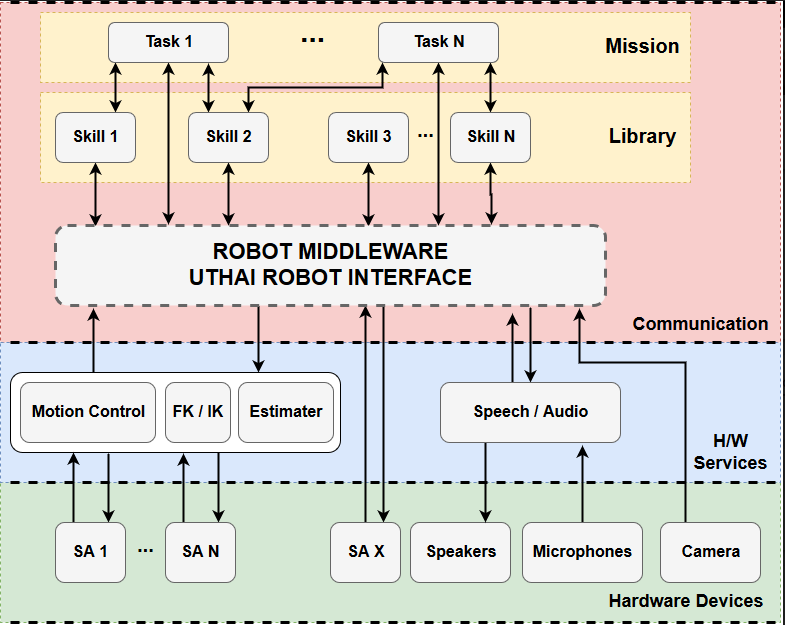
\includegraphics[width=0.8\textwidth]{chapter3/images/uthai_diagram.png}
	\caption{โครงสร้างพื้นฐานของหุ่นยนต์อุทัย}
	\label{fig:uthai_diagram}
\end{figure}

\clearpage
\subsection{ออกแบบสถาปัตยกรรมของหุ่นยนต์}
หลักการออกแบบสถาปัตยกรรมของหุ่นยนต์ฮิวมานอยด์ UTHAI จะออกแบบระบบให้อยู่บนระบบพื้นฐาน ROS
เนื่องจากการใช้กรอบการทำงานที่มีประสิทธิภาพ และความยืดหยุ่นสูง จะช่วยทำให้สามารถปรับเปลี่ยนระบบการควบคุมของหุ่นยนต์ฮิวมานอยด์ได้ง่ายและรวดเร็ว
ดังนั้นแล้วผู้วิจัยจึงได้แบ่งการประมวลผลออกเป็น 2 ส่วนคือ
\begin{enumerate}[label=\arabic*, leftmargin=1.5cm]\setlength\itemsep{-0.25em}
	\item หน่วยประมวลผลควบคุมระดับสูง (High Level Controller)
	\item หน่วยประมวลผลควบคุมระดับต่ำ (Low Level Controller)
\end{enumerate}
\begin{figure}[!ht]
	\centering
	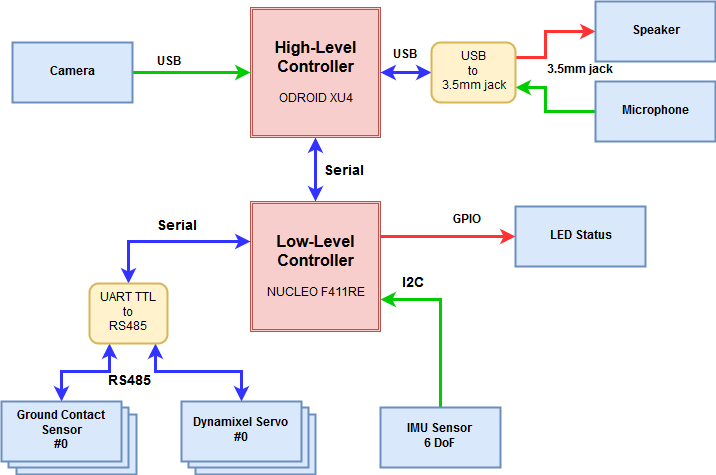
\includegraphics[width=0.8\textwidth]{chapter3/images/uthai_argitec.png}
	\caption{สถาปัตยกรรมของหุ่นยนต์ฮิวมานอยด์ UTHAI}
	\label{fig:uthai_argitec}
\end{figure}

\clearpage
\subsubsection{หน่วยประมวลผลควบคุมระดับสูง (High level controller)}
ระบบควบคุมหลักของหุ่นยนต์ UTHAI นั้นจะอยู่ที่หน่วยประมวลผลขั้นสูง ใช้เป็นบอร์ดคอมพิวเตอร์ ODROID-XU4 ตัวประมวลผลหลักนี้
มีหน้าที่ในการทำการคำนวณ เส้นทางการเดินของหุ่นยนต์ให้มีเสถียรภาพ ตรวจการขัดกันของโครงสร้างของหุ่นยนต์
รวมไปถึงรับค่าข้อมูลภาพจากกล้อง และข้อมูลเสียงจากไมโครโฟนมาประมวลผล หลังจากนั้นจะทำการนำค่าทั้งหมดที่ได้จากการคำนวณ
มาแปลงให้อยู่ในรูปของชุดข้อมูล แล้วส่งออกไปให้ระบบกลาง (ROS) ในการส่งต่อไปให้อุปกรณ์อื่นต่อไป

\begin{figure}[ht]
	\centering
	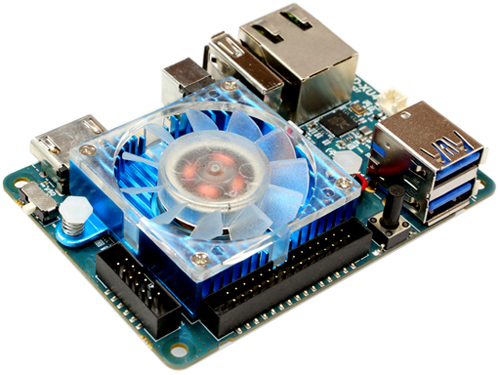
\includegraphics[width=0.45\textwidth]{chapter3/images/odroid_xu4.jpeg}
	\caption{บอร์ดคอนโทรลเลอร์ Odroid XU4}
	\label{fig:controller_xu4}
\end{figure}

\subsubsection{หน่วยประมวลผลควบคุมระดับต่ำ (Low level controller)}
ระบบควบคุมขั้นต่ำเป็นหน่วยประมวลผลที่รองลงมาจาก บอร์ดคอมพิวเตอร์ โดยใช้บอร์ดไมโครคอลโทรเลอร์ Nucleo F411RE
เป็นหน่วยประมวลผลขั้นต่ำ สำหรับในการติดต่อกับอุปกรณ์อิเล็กทรอนิกส์ต่าง ๆ ที่อยู่ภายในตัวของหุ่นยนต์ เช่น
ค่าเซนเซอร์ที่ฝ่าเท้าซึ่งสามารถบอกได้ว่าควรใช้สมการไหนในการคำนวณพลวัต หรือค่าของเซนเซอร์ IMU มีความสำคัญมาก
ในการทำให้หุ่นยนต์ฮิวมานอยด์เดินได้อย่างมีเสถียรภาพ เมื่ออ่านค่าเซนเซอร์ต่างๆได้แล้ว
หน่วยประมวลผลขั้นต่ำจะนำค่าที่ได้จากการอ่านเซนเซอร์เหล่านี้แปลงให้อยู่ในลักษณะของชุดข้อมูล แล้วส่งออกไปในระบบกลาง(ROS)
นอกเหนือจากนี้หน่วยประมวลผลขั้นต่ำยังทำหน้าที่รับค่าคำสั่งมาจากระบบกลาง ในการสั่งงานให้หุ่นยนต์มีท่าทางต่าง ๆตามต้องการได้

\begin{figure}[ht]
	\centering
	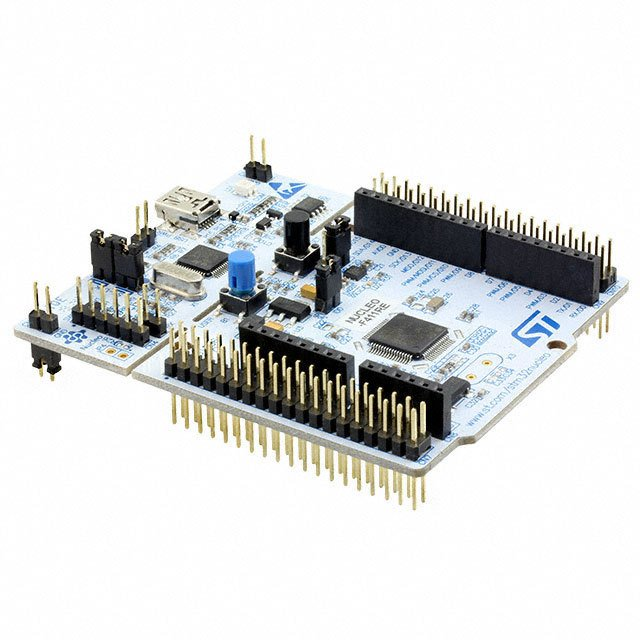
\includegraphics[width=0.45\textwidth]{chapter3/images/nucleo_f411re.jpeg}
	\caption{บอร์ดคอนโทรลเลอร์ Nucleo F411RE}
	\label{fig:controller_f411re}
\end{figure}


%%%%%%%%%%%%%%%%%%%%%%%%%%%%%%%%%%%%%%%%%%%%%%%%%%%%%%%%%%%%%%%%%%%%%%%%%%%%%%%




\clearpage
\subsection{จัดทำคู่มือและเอกสารการใช้งาน}
คู่มือจะเป็นส่วนที่ผู้มาพัฒนาต่อยอดสามารถที่จะอ่านทำความเข้าใจได้ โดยจะเขียนให้อยู่ในรูปของไฟล์ 
Markdown (.md) และเก็บเอาไว้ในเว็บไซท์ GitHub ซึ่งเป็นแหล่งรวม Source code ออนไลน์
สามารถเข้าไปดาวน์โหลดไฟล์ลงเครื่องผู้ใช้ แล้วทำการติดตั้งใช้งานได้เลย อีกทั้งผู้ใช้ยังสามารถส่ง Code
ของตัวเองเข้าระบบเพื่อเพิ่มประสิทธิภาพในการทำงานของโปรแกรม

ส่วนที่เน้นในการทำคู่มือคือ\vspace{-5mm}
\begin{enumerate}[label=\arabic*, leftmargin=1.5cm]\setlength\itemsep{-0.25em}
	\item รายการวัสดุที่ใช้ในการทำหุ่นยนต์ฮิวมานอยด์ UTHAI
	\item รายระเอียดการเชื่อมต่อระหว่างอุปกรณ์ที่อยู่ในตัวหุ่นยนต์
	\item รายระเอียดการประกอบชิ้นส่วนทางกล
	\item รายละเอียดการใช้งานโปรแกรมพื้นฐาน
\end{enumerate}

\subsubsection{รายการวัสดุที่ใช้ในการทำหุ่นยนต์ฮิวมานอยด์ UTHAI}
\begin{table}[ht]
	\centering
	\begin{tabular}{| l | c | c | c|}
		\hline
		รายการ & จำนวน(หน่วย) & ราคา/หน่วย(บาท) & ราคารวม(บาท) \\
		\hline
		===== Processing Unit & - & - & -\\
		Odroid XU4 Embeded Computer & 1 & 3800 & 3800\\
		Shifter Shield for Odoird XU4 & 1 & 1000 & 1000\\
		===== Sensor & - & - & -\\
		Force sensitive Resistor & 8 & 300 & 2400\\
		Electronic Component & 1 & 2000 & 2000\\
		MPU9255 9 Axis IMU Module & 1 & 500 & 500\\
		===== Structure & - & - & -\\
		อุปกรณ์ส่งกำลัง & 1 & 3000 & 3000\\
		ค่าวัสดุ เช่น Filament 3D printer , Carbon Fiber & 1 & 8000 & 8000\\
		สปริง & 14 & 50 & 700\\
		อุปกรณ์สิ้นเปลือง เช่น กระดาษทราย ฯลฯ & 1 & 1000 & 1000\\
		===== อุปกรณ์เสริม Motor Dynamixel & - & - & -\\
		Frame สำหรับต่อพ่วงมอเตอร์ & 4 & 2000 & 8000\\
		Horn Bearing & 4 & 1400 & 5600\\
		อุปกรณ์จ่ายพลังงาน & - & - & -\\
		Power Supply & 1 & 2000 & 2000\\
		Battery Li-Po 4 cell & 1 & 3000 & 3000\\
		===== รวม & - & - & 48000\\
		\hline
	\end{tabular}
	\caption{ตารางแสดงรายการของวัสดุต่าง ๆ}
	\label{tab:matrial_buyer}
\end{table}
ใช้สำหรับแจกแจงค่าใช้จ่ายเบื้องต้นเท่านั้น ไม่สามารถใช้อ้างอิงงบประมาณแบบละเอียดได้

%%%%%%%%%%%%%%%%%%%%%%%%%%%%%%%%%%%%%%%%%%%%%%%%%%%%%%%%%%%%%%%%%%%%%%%%%%%%%%%
\clearpage
\subsection*{UTHAI-Tools}
เครื่องมือสำหรับการทำงานในฮิวมานอยด์

\subsubsection*{sketch-lib}
เป็นเครื่องมือที่ใช้สำหรับเอาไว้วาดรูปเฟรมของหุ่นยนต์

\begin{figure}[ht]
	\centering
	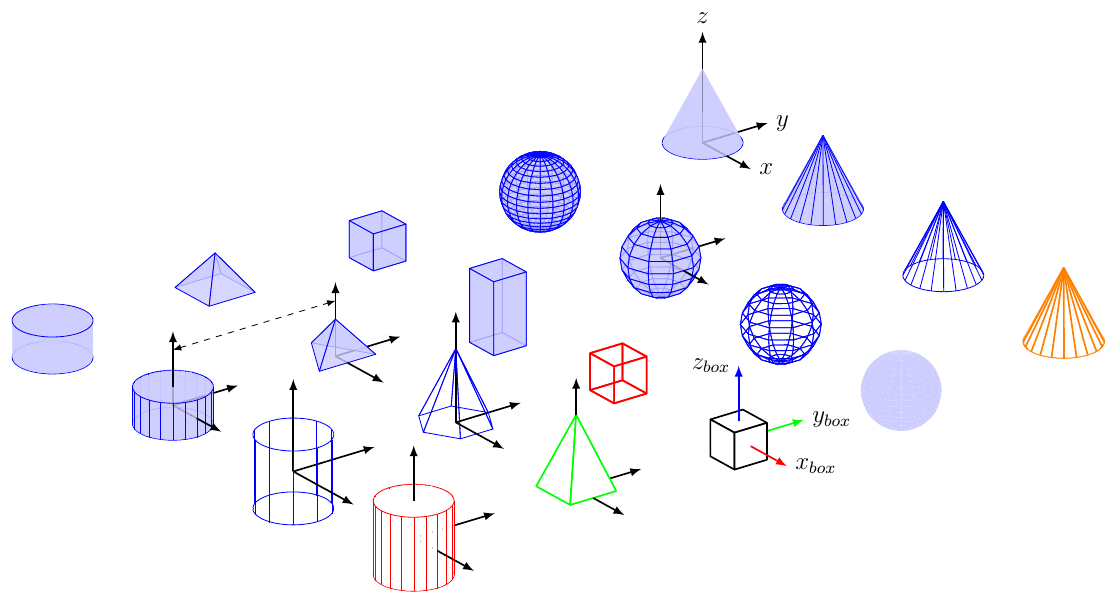
\includegraphics[width=0.7\textwidth]{chapter3/images/basic-shapes.png}
	\caption{ภาพตัวอย่างการวาดออฟเจ็คต่างๆ}
	\label{fig:basic-shapes_sk}
\end{figure}
\begin{figure}[ht]
	\centering
	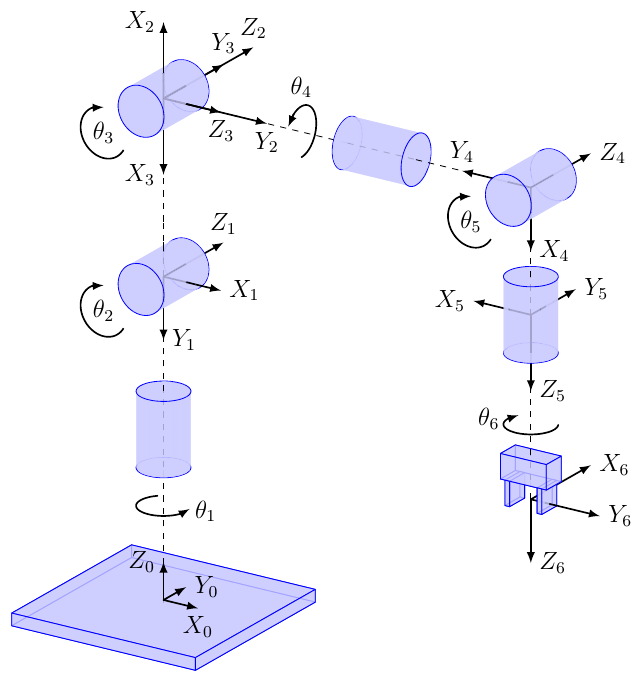
\includegraphics[width=0.5\textwidth]{chapter3/images/test_robot.png}
	\caption{ภาพตัวอย่างการวาดเฟรมของแขนกล}
	\label{fig:test-robot_sk}
\end{figure}
\begin{figure}[ht]
	\centering
	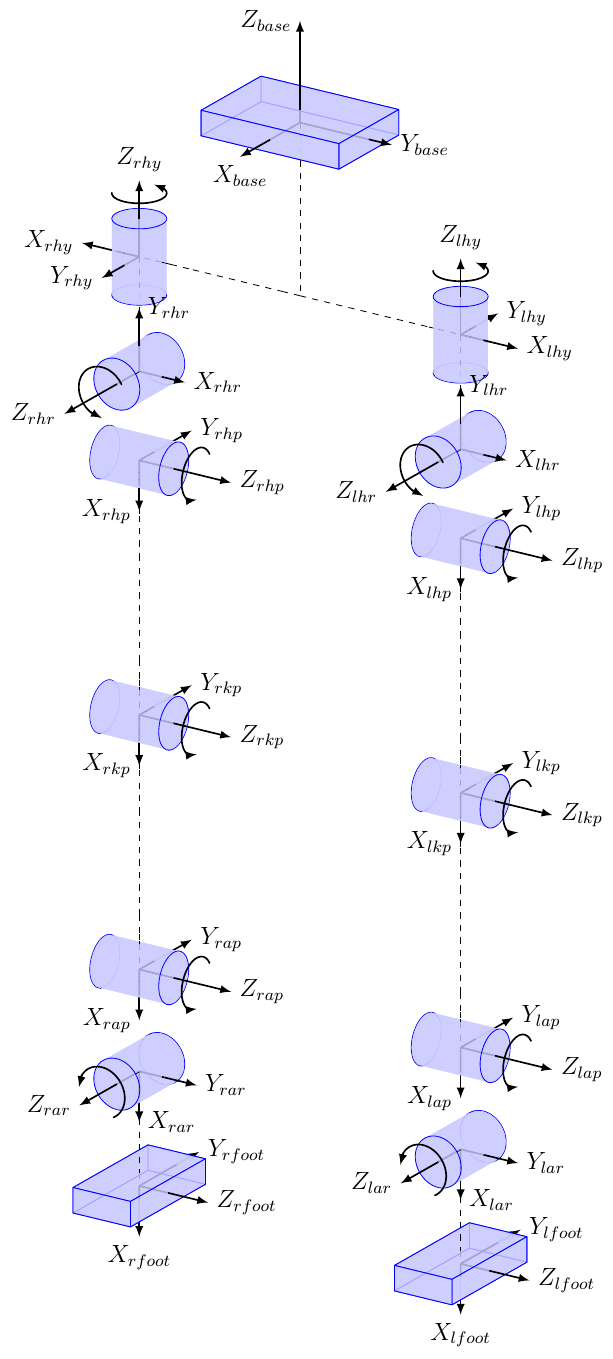
\includegraphics[width=0.4\textwidth]{chapter3/images/uthai_kinematics.png}
	\caption{ภาพตัวอย่างการวาดเฟรมของหุ่นยนต์ฮิวมานอยด์}
	\label{fig:uthai_kinematics_sk}
\end{figure}
